\documentclass[11pt]{beamer}

% Beamer style
%\usetheme[secheader]{Madrid}
% \usetheme{CambridgeUS}
\useoutertheme{infolines}
\usecolortheme[rgb={0.65,0.15,0.25}]{structure}
% \usefonttheme[onlymath]{serif}
\beamertemplatenavigationsymbolsempty
%\AtBeginSubsection

% Packages
\usepackage[latin1]{inputenc}
\usepackage{color}
\usepackage{amsmath, amsfonts, amssymb}
\usepackage{marvosym}
\usepackage{graphicx}
% \usepackage{epsfig}
\usepackage{/home/robin/LATEX/Biblio/astats}

% Commands
\definecolor{darkred}{rgb}{0.65,0.15,0.25}
\definecolor{darkgreen}{rgb}{0,0.4,0}
\newcommand{\emphase}[1]{\textcolor{darkred}{#1}}
\newcommand{\Esp}{\mathbb{E}}
\newcommand{\dd}{\text{d}}
% \newcommand{\emphase}[1]{{#1}}
\newcommand{\paragraph}[1]{\textcolor{darkred}{#1}}
\newcommand{\refer}[1]{\textcolor{gray}{\footnotesize{[\cite{#1}]}}}
\newcommand{\Refer}[1]{\textcolor{gray}{\footnotesize{[#1]}}}
\newcommand{\ra}{$\emphase{\rightarrow} \;$}
\newcommand{\fighd}{../FIGURES}
\newcommand{\fignet}{../../../RESEAUX/EXPOSES/FIGURES}

% Names
\newcommand{\chr}{}
\newcommand{\comment}{}
\newcommand{\Pt}{{\widetilde{P}}}
\newcommand{\St}{{\widetilde{S}}}
\newcommand{\Zt}{{\widetilde{Z}}}
\newcommand{\mt}{{\widetilde{m}}}

\newtheorem{proposition}{\normalsize Proposition}

%====================================================================
\title[Detecting genomic alterations]{Detection of (recurrent) genomic alterations: \\ Adapting statistics to data dimension}

\author[S. Robin]{S. Robin}

\institute[INRA / AgroParisTech]{
  \bigskip
 \begin{tabular}{ccccc}
    
\includegraphics[height=.075\textheight]{../FIGURES/LogoINRA-Couleur} & 
    \hspace{.02\textwidth} &
    
\includegraphics[height=.075\textheight]{../FIGURES/logagroptechsolo} & 
    \hspace{.02\textwidth} &
    
\includegraphics[height=.075\textheight]{../FIGURES/logo-ssb} \\ 
  \end{tabular} \\
  \bigskip
%   {\footnotesize
%   \begin{tabular}{l}
%   Joint (on-going) work with \\ 
%   1 -- A. Cleynen, E. Lebarbier, F. Picard, G. Rigaill, \\
%   2 -- L. Decreusefond, M.-P. Etienne, G. Lang, V. Stefanov, P. Vallois
%   \end{tabular} \\~
% %     \begin{tabular}{rll}
% %     On-going work with & L. Decreusefond, & M.-P. Etienne, \\
% %     & G. Lang, & V. Stefanov \\
% %     \end{tabular}
%     }
  }

  \date[IBM, Dec. 2015]{Horizon des math�matiques, IBM, Dec.'15}

%====================================================================

%====================================================================
%====================================================================
\begin{document}
%====================================================================
%====================================================================
\frame{\titlepage}
  
%====================================================================
\section*{Genomic alterations}
\frame{\frametitle{Genomic alterations}
}
  
%====================================================================
\frame{\frametitle{Genomic alterations}
  Genomic alterations are associated with (responsible for?) various
  types of cancers.  
  $$
  \begin{tabular}{cc}
    \onslide+<1->{Normal cell} & \onslide+<2->{Tumor cell} \\
    \onslide+<1->{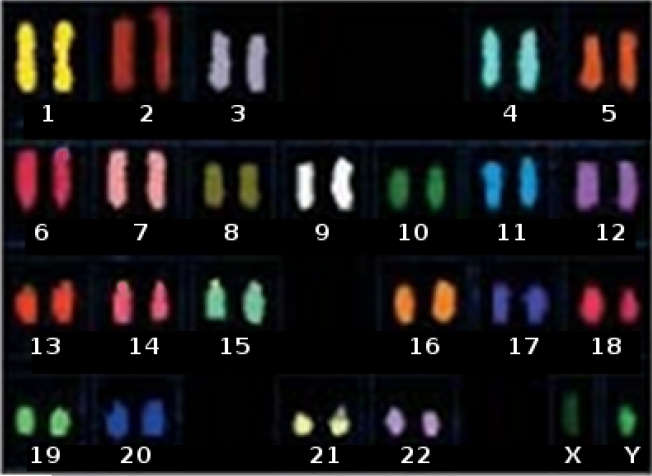
\includegraphics[height=.4\textheight]{../FIGURES/Hup08-Fig121b}}
    &
    \onslide+<2->{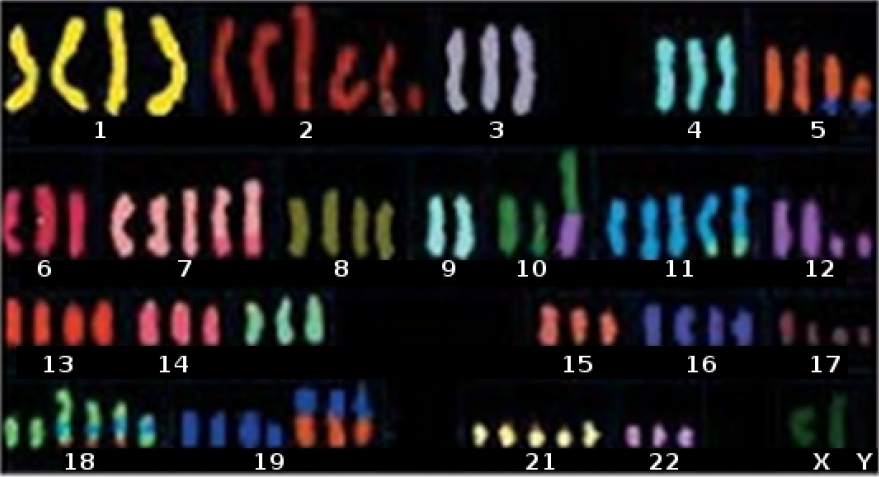
\includegraphics[height=.4\textheight]{../FIGURES/Hup08-Fig121a}}
  \end{tabular}
  $$
  \refer{Hup08}
}

%====================================================================
\frame{\frametitle{Different technologies 1/2}

  \paragraph{Micro-arrays:} from $10^2$ to $10^4$ probes / chromosome
  $$
  \begin{tabular}{cc}
    \onslide+<2->{CGH profile} & \onslide+<1->{Tumor cell} \\
    \onslide+<2->{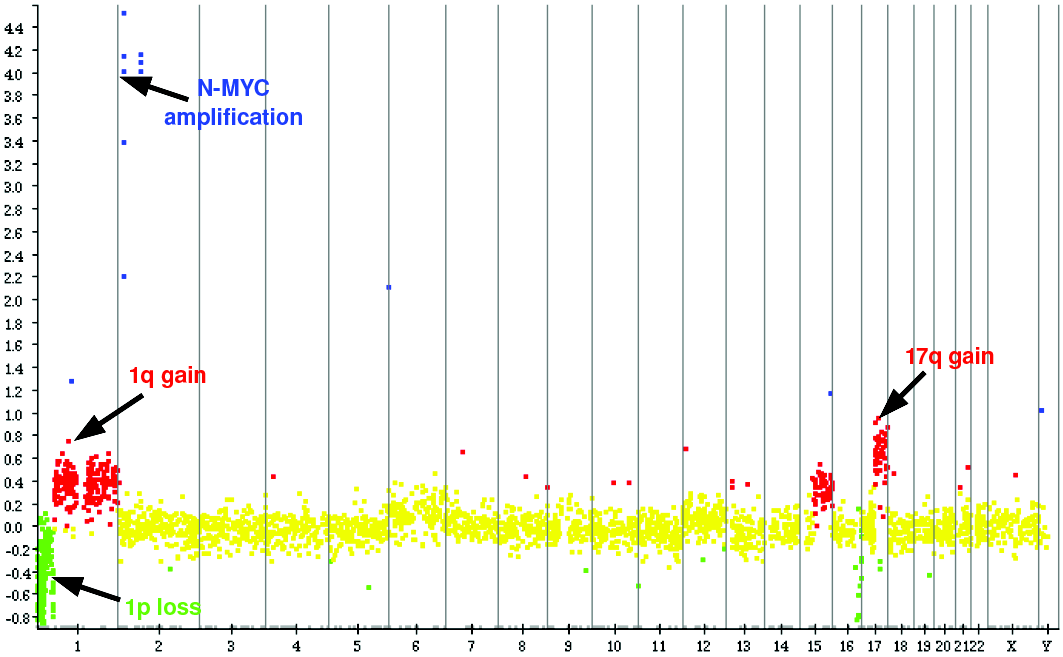
\includegraphics[height=.43\textheight]{../FIGURES/Hup08-Fig128a}}
    &
    \onslide+<1->{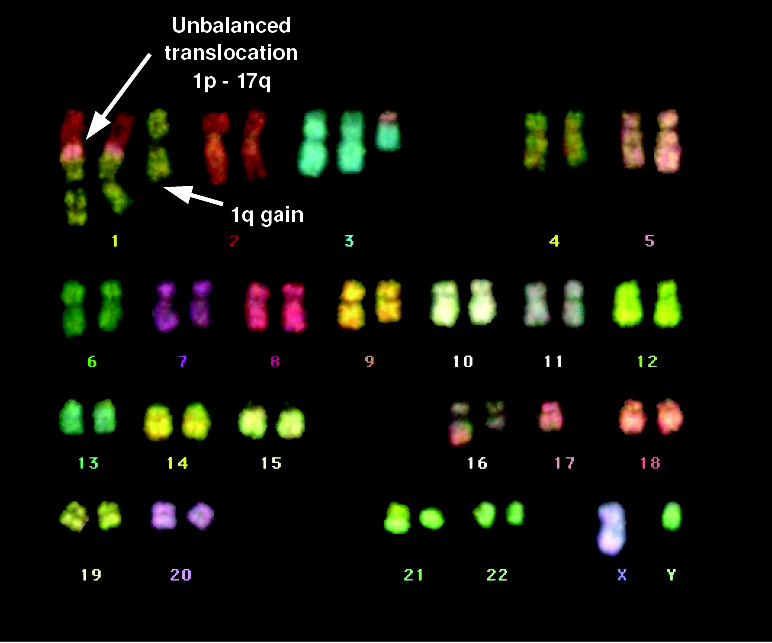
\includegraphics[height=.43\textheight]{../FIGURES/Hup08-Fig128b}}
  \end{tabular}
  $$
  \onslide+<2->{\paragraph{Data:}
  $
  Y_t = \text{(fluorescence) signal at probe $t$}
  $}
}


%====================================================================
\frame{\frametitle{Different technologies 2/2}

  \paragraph{Next generation sequencing (NGS):} from $10^6$ to $10^8$ nucleotides / chromosome \\~
  
  \pause 
  \begin{itemize}
   \item DNAseq reads are mapped along a reference genome. 
   \item Variation of there density reveals variation of the copy number \refer{RGI12}.
  \end{itemize}
  
  $$
  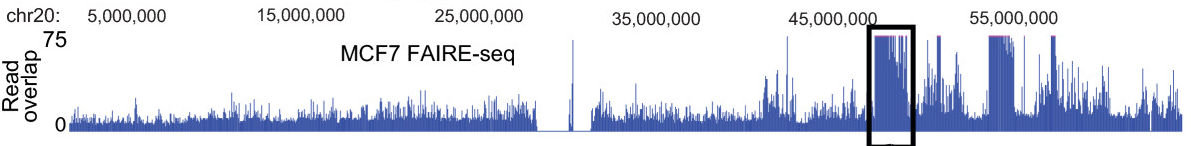
\includegraphics[width=1\textwidth]{../FIGURES/RGI12-Fig4c}
  $$
  

  \bigskip
  \paragraph{Data:}
  $$
  Y_t = \text{number of mapped reads starting at nucleotide $t$}
  $$	
}

%====================================================================
\frame{\frametitle{Biological questions}

   \paragraph{Detection:} \textcolor{gray}{How many change-points?} 
   
   \bigskip
   \paragraph{Location:} Where are the change-points? 
   
   \bigskip
   \paragraph{Precision:} How precise is the inferred location? 
   
   \bigskip
   \paragraph{Sample comparison:} Are they located at the same locus in two different samples?
   
   \bigskip
   \paragraph{Recurrent alterations:} Are some alterations especially frequent in a given set of patients?
}

%====================================================================
\frame{\frametitle{Statistical issues}

  \paragraph{Modeling:} 
  \begin{itemize}
   \item Account for the type of data: CGH data = real numbers, DNAseq data = counts
   \item Independence of data collected at each locus (probe, nucleotide)?
   \item Which joint model for a set of CNV profiles?
  \end{itemize} 
  
  \bigskip
  \paragraph{Algorithmics:} 
  \begin{itemize}
   \item Need to answer the question (e.g. retrieve the optimal solution)
   \item With computational efficiency (i.e. use scalable algorithms)
  \end{itemize} 

  \bigskip
  \paragraph{Model selection:} 
  \begin{itemize}
   \item \textcolor{gray}{Estimating the number of change-points}
  \end{itemize} 
  
}

%====================================================================
\frame{\frametitle{Outline}
  \tableofcontents
}

%====================================================================
\section[Detecting alterations]{Detecting alterations: Algorithmic issues}
\frame{\frametitle{Detecting alterations}
}
  
%====================================================================
\frame{\frametitle{Change-point problems in genomics} 
% %====================================================================
% \frame{\frametitle{A change-point detection problem}

  \bigskip
  \begin{tabular}{l}
    \vspace{-.05\textheight}
    \paragraph{Comparative genomic hybridization:} microarrays / copy number variation \\
    \begin{tabular}{c}
	 \begin{overprint}
	   \onslide<1>
	   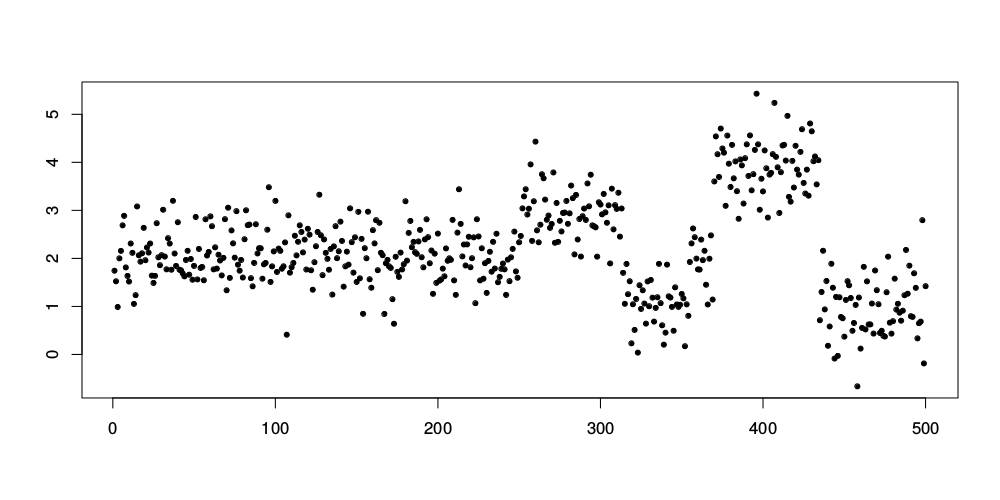
\includegraphics[height=.45\textheight, width=.9\textwidth]{../FIGURES/FigSeg-Cambridge-CGH}
	   \onslide<2>
	   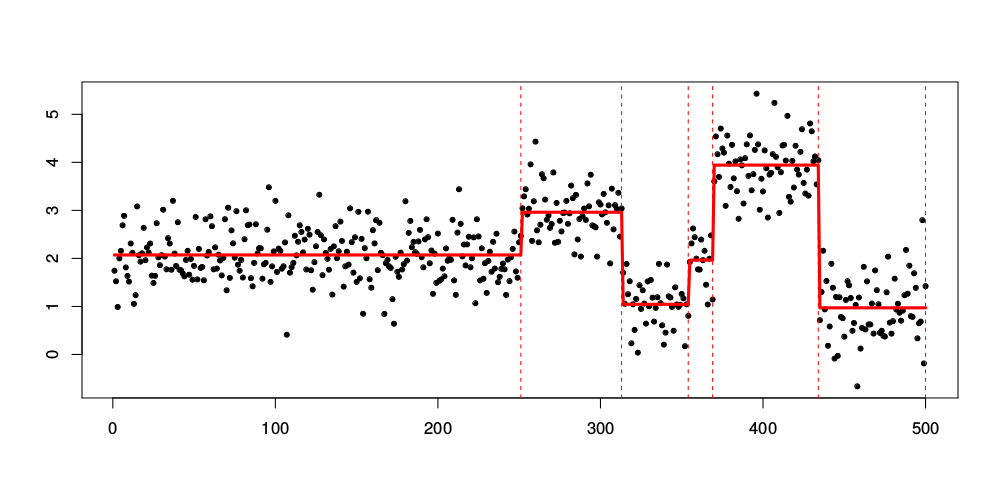
\includegraphics[height=.45\textheight, width=.9\textwidth]{../FIGURES/FigSeg-Cambridge-CGH-seg}
	 \end{overprint}
    \end{tabular}
    \\
    \vspace{-.05\textheight}
    \paragraph{RNA-sequencing:} massive sequencing / gene expression \\
    \begin{tabular}{c}
	 \begin{overprint}
	   \onslide<1>
	   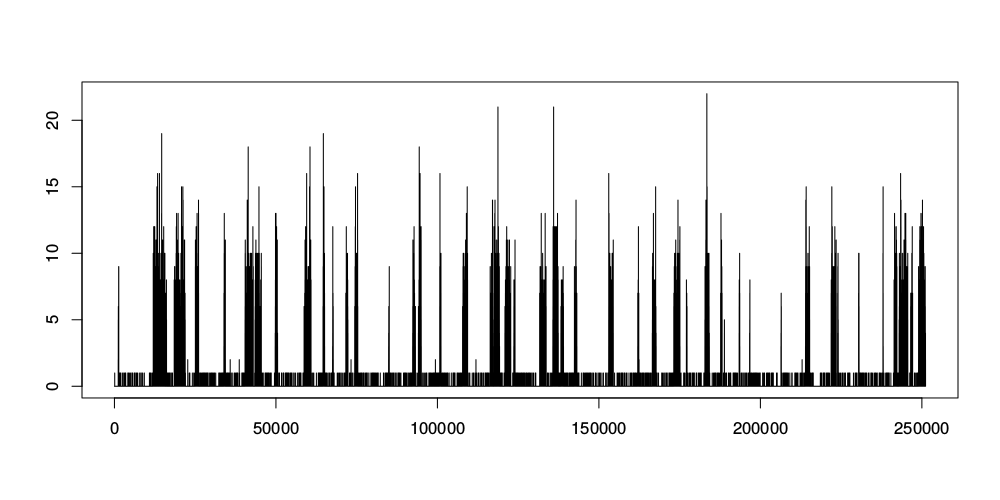
\includegraphics[height=.45\textheight, width=.9\textwidth]{../FIGURES/FigSeg-Cambridge-RNAseq}
	   \onslide<2>
	   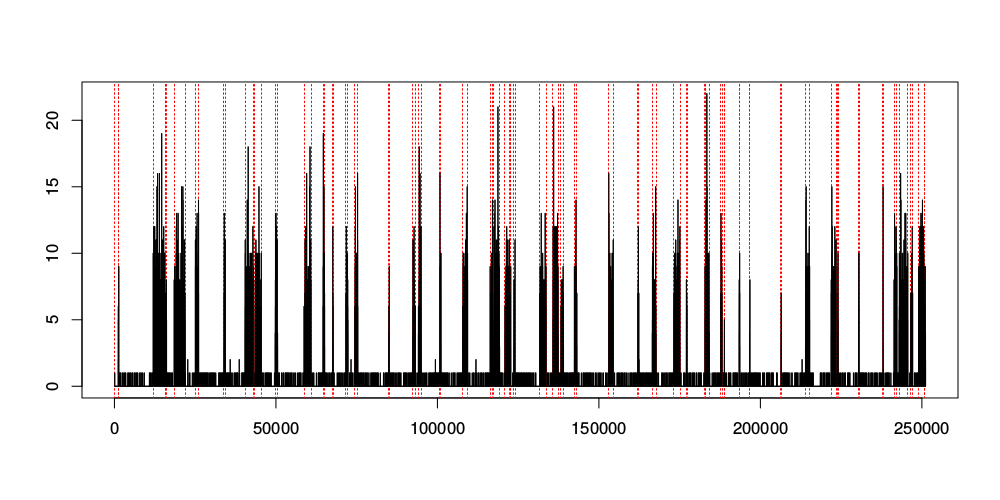
\includegraphics[height=.45\textheight, width=.9\textwidth]{../FIGURES/FigSeg-Cambridge-RNAseq-seg}
    \end{overprint}
    \end{tabular}
  \end{tabular}
}

% %====================================================================
% \frame{\frametitle{Change-point problems in genomics} 
% 
%   \paragraph{Genomic data} are often collected 'along the genome', similarly to time series
%   
%   \bigskip \bigskip
%   \paragraph{Genomic experiments} often aim at finding regions in which some specific event occurs:
%   \begin{itemize}
%    \item copy number variations (gain or loss of genomic regions: CGH, DNAseq)
%    \item gene detection (detection of transcribed region: microarrays, RNAseq)
%    \item protein-DNA interactions (e.g. detection of protein biding sites: ChIP-chip, ChIPseq)
% %    \item DNA-DNA interactions (e.g. chromosomal territories: 3C, HiC)
%    \item ...
%   \end{itemize}
% 
% %   \bigskip \medskip
% %   \paragraph{Genomic technologies} now provide information at the nucleotide resolution
%   }

%====================================================================
\frame{\frametitle{Basic change-point detection model}

  \begin{tabular}{cc}
    \hspace{-.05\textwidth}
    \begin{tabular}{p{.5\textwidth}}
      \onslide+<2->{\paragraph{Statistical model.} 
        \begin{itemize}
        \item $\text{Signal} = f(\text{Position})$; \\}
        \onslide+<3->{
        \item Breakpoint positions: \\
          $\tau_1, \tau_2, ..., \tau_{K-1};$ \\}
        \onslide+<4->{
        \item 'Mean' signal within each region: \\
          $\theta_1, \theta_2, ..., \theta_K$; \\}
        \onslide+<5->{
        \item Observed signal at time $t$: \\
          independent variables
        \end{itemize}}
    \end{tabular}
    & 
    \hspace{-.1\textwidth}
    \begin{tabular}{c}
      \onslide+<2->{
        \hspace{-.5\textwidth}
        \onslide+<3->{if $t \in \textcolor{blue}{r_k}$,} \quad $Y_t$
        \onslide+<5->{$\sim
          F($}\onslide+<4->{$\textcolor{red}{\theta_k}$}\onslide+<5->{$)$}
        \\}
      \begin{overprint}
        \onslide<2>
%        $\qquad \qquad \;\;\, Y_t =$ \\
        \includegraphics[width=.5\textwidth, height=.7\textheight]{../FIGURES/FigSeg-Budapest-1}
        \onslide<3>
%        if $t \in \textcolor{blue}{r_k}, \quad Y_t$ \\
        \includegraphics[width=.5\textwidth, height=.7\textheight]{../FIGURES/FigSeg-Budapest-2}
        \onslide<4>
%        if $t \in \textcolor{blue}{r_k}, \quad Y_t \textcolor{red}{\theta_k}$ \\
        \includegraphics[width=.5\textwidth, height=.7\textheight]{../FIGURES/FigSeg-Budapest-3}
        \onslide<5>
%        if $t \in \textcolor{blue}{r_k}, \quad Y_t \sim
%        \Fcal(\textcolor{red}{\theta_k})$ \\ 
        \includegraphics[width=.5\textwidth, height=.7\textheight]{../FIGURES/FigSeg-Budapest-4}
        \onslide<6->
%        if $t \in \textcolor{blue}{r_k}, \quad Y_t \sim
%        \Fcal(\textcolor{red}{\theta_k})$ \\ 
        \includegraphics[width=.5\textwidth, height=.7\textheight]{../FIGURES/FigSeg-Budapest-0}
      \end{overprint}
    \end{tabular}
  \end{tabular}

}

%=========================================================================
\frame{\frametitle{Inference problem}

  \paragraph{Two different types of parameters:}
  \begin{itemize}
  \item Segmentation (change-point locations): 
%   $T = (\tau_1, \dots, \tau_{K-1})$ \\
  $\tau_1, \dots, \tau_{K-1}$ \\
    \ra \emphase{discrete} parameters;
  \item Distribution parameters (within segment means): 
%   $\theta = (\theta_1, \dots, \theta_K)$ \\
  $\theta_1, \dots, \theta_K$ \\
    \ra \emphase{continuous} parameters.
  \end{itemize}

%   \bigskip \bigskip \pause
%   \paragraph{Most common strategy: Maximum likelihood.}
%   To get estimate of the parameters of this model ($T, \theta$)
%   we choose to maximize the likelihood of the observed data:
%   \begin{eqnarray*}
%   p(Y; T, \theta) & = & \prod_{\textcolor{red}{r_k}} \prod_{t \in r_k} p(Y_t; \textcolor{blue}{\theta_k}) \\
%   \Rightarrow \qquad \log p(Y; T, \theta) & = & \sum_{\textcolor{red}{r_k}}
%   \sum_{t \in r_k} \log p(Y_t ;\textcolor{blue}{\theta_k}).
%   \end{eqnarray*}
%   }
  
% %====================================================================
% \frame{\frametitle{Parameter inference} 

  \pause\bigskip
  \paragraph{When the change-points are known,} estimating the
  parameters is (generally) an easy task, e.g. 
  $$
  \widehat{\theta}_k = \text{mean value of the signal within the region}
  $$

  \pause\bigskip
  \paragraph{Finding the breakpoints:} 
%   We now have to find the change-points $\tau_1$, \dots, $\tau_{K-1}$ that maximize the log-likelihood
%   $$
%   \log p(Y; T) = \sum_{\textcolor{red}{r_k}}  \sum_{t \in r_k} \log p(Y_t ;\widehat{\theta}_k), 
%   \qquad
%   r_k = [\tau_{k-1}+1; \tau_{k}]
%   $$
%   
%   \pause\bigskip
%   \paragraph{Problem.}
  The number possible choices for the change-points grows exponentially:
  $$
  n=1\,000 \text{ loci}, \qquad K = 20 \text{ regions} \quad \longrightarrow \quad
  \binom{n-1}{K-1} \simeq 10^{40}
  $$
  \ra Impossible to explore for large $n$ and $K$

\label{Page:ParamInfer}}

%====================================================================
\frame{\frametitle{Shortest path problem}

  \paragraph{Cost of segment.} Define the cost of segment $r= [i, j]$, 
%   as
%   $$
%   C(i, j) = \sum_{t \in [i, j]} - \log p(Y_t; \widehat{\mu}_{[i, j]}),    
%   $$
  e.g.
  $$
  C(i, j) = \sum_{t \in [i, j]} (Y_t - \widehat{\theta}_{[i, j]})^2,    
  $$
  \pause
  finding the maximum likelihood segments
%   the maximization of
%   $$
%   \log p(\Ybf; T) = \sum_k  \sum_{t \in r_k} \log p(Y_t; \widehat{\mu}_k).
%   $$
  can be restated as a \emphase{shortest path problem}, that is to find the path
%   \begin{itemize}
%   \item going from 1 to $n$,
%   \item in $K$ steps,
%   \item for the best possible cost: 
  that is solution of 
  $$
  \min_{\tau_1 < \tau_2 < \dots <  \tau_{K-1}}
  C(1, \tau_1) + C(\tau_1+1, \tau_2) + ... + C(\tau_{K-1}+1, n).
  $$
%   \end{itemize}
%   \bigskip \pause
%   \paragraph{Examples: }
%   \begin{eqnarray*}
%     \text{CGHarray:} \qquad C(i, j) & = & \sum_{t \in [i, j]} \left(Y_t - \overline{Y}_{[i, j]}\right)^2, \\
%     \text{DNAseq:} \qquad C(i, j) & = & - \sum_{t \in [i, j]} Y_t \log\left(\overline{Y}_{[i, j]}\right)
%   \end{eqnarray*}
%   }

% %====================================================================
% \frame{\frametitle{Dynamic programming algorithm}

%   \paragraph{Principle.} 
  \pause \bigskip 
  \paragraph{Dynamic programming principle:} 
  {\sl Sup-paths of the optimal paths are optimal  themselves.}

  \pause \bigskip 
  \paragraph{Algorithm.} 
%   $S_K(i, j) =$ cost of the optimal segmentation of series $[i, j]$ into $K$ segments:
%   \begin{eqnarray*}
%     S_2(i, j) & = & \min_{t \in [i, j-1]} C(i, t) + C(t+1, j) \\
%     S_K(i, j) & = & \min_{t \in [i, j-1]} S_{K-1}(i, t) + C(t+1, j) 
%   \end{eqnarray*}
%   A second (backward) recursion provides the boundaries of the optimal segments.
  A forward-backward recursion provides the segmentation with minimal cost with complexity $O(K n^2)$ in time and $O(Kn)$ in space.
  
%   \pause \bigskip 
%   \paragraph{Complexity:} $O(K n^2)$ for computational time and $O(Kn)$ for memory space.
 }

%====================================================================
\frame{\frametitle{Comparative study for SNP arrays}

  \bigskip
  \paragraph{Benchmark of manually annotated profiles:} ROC curves \refer{Hoc12}
  $$
  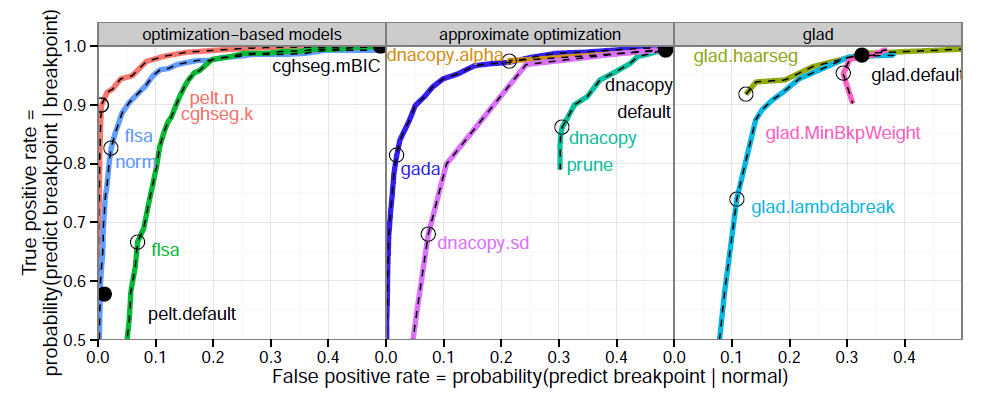
\includegraphics[width=\textwidth]{../FIGURES/Hoc12-Fig3-3}     
  $$
  \vspace{-0.05\textheight}
  \begin{itemize}
   \item Earlier work with similar conclusions: \refer{LJK05}
   \item Improvements for model selection: \refer{ZhS07,ClL14}
  \end{itemize}

  
 }

%====================================================================
\frame{\frametitle{Location of the change-points}

  \paragraph{Dynamic programming} provides the optimal segmentation but no information about the precision of their location.
  
  \bigskip \bigskip
  \paragraph{Bayesian setting.} 
  \begin{itemize}
   \item A Bayesian version of the segmentation model exists.
   \item The posterior distribution of a given change point $p(\tau_k | Y)$ can be considered
   \item And computed using a dynamic programming trick, changing 
   $$
   \min \rightarrow \sum, 
   \qquad
   + \rightarrow \times. 
   $$
  \end{itemize}
  \refer{RLR11,ClR14}
}

%====================================================================
\frame{\frametitle{Posterior distribution of transcript boundaries in yeast}

  \vspace{-.05\textheight}
  \begin{tabular}{p{.2\textwidth}p{.7\textwidth}}
    \begin{tabular}{p{.3\textwidth}}
	 One gene \\
	 (with 2 exons) \\
	 \\
	 $\times$ \\
	 \\
	 Three growth \\
	 conditions: 
	 $A$, $B$, $C$
    \end{tabular}
    &
    \begin{tabular}{p{.7\textwidth}}
    \includegraphics[width=.7\textwidth]{../FIGURES/compyeastresult.pdf}
    \end{tabular}
  \end{tabular}
}

%====================================================================
\frame{\frametitle{Comparing transcript boundaries in yeast}

3 comparisons ($A-B$, $A-C$, $B-C$) $\times$ 4 boundaries:
  
\centerline{\includegraphics[width=.8\textwidth, height=.8\textheight]{../FIGURES/cred-yeast.pdf}}
}

%====================================================================
\frame{\frametitle{Fastening the DP algorithm}

  \paragraph{Quadratic complexity} $O(Kn^2)$ is not acceptable for very
  large signals ($n = 10^8$).

  \pause\bigskip
  \paragraph{Dynamic programming} uses 
  a recursion
%   the recursion
%   $$
%   S_K(1, j) = \min_t S_{K-1}(1, t) + C(t+1, j)
%   $$
  that relies on past optimal solutions.

  \pause \bigskip
  \paragraph{Pruning the search.} When going along the genome, it turns out that some past solutions will never contribute to the global optimum
  \begin{itemize}
  \item either by comparing their respective cost functions \refer{Rig10,CKL14}
  \item or because of the penalty to be used for model selection \refer{KFE11}.
  \end{itemize} 
  ~ \\
  The computational time is reduced to $O(K n \log n)$ for \refer{Rig10} to $O(n)$ for \refer{KFE11}. 
  }

%====================================================================
\section[Detecting recurrent alterations]{Detecting recurrent alterations: Probabilistic issues}
\frame{\frametitle{Detecting recurrent alterations}}
  
%====================================================================
\frame{\frametitle{Recurrent alterations}

  \vspace{-.05\textheight}
  $$
  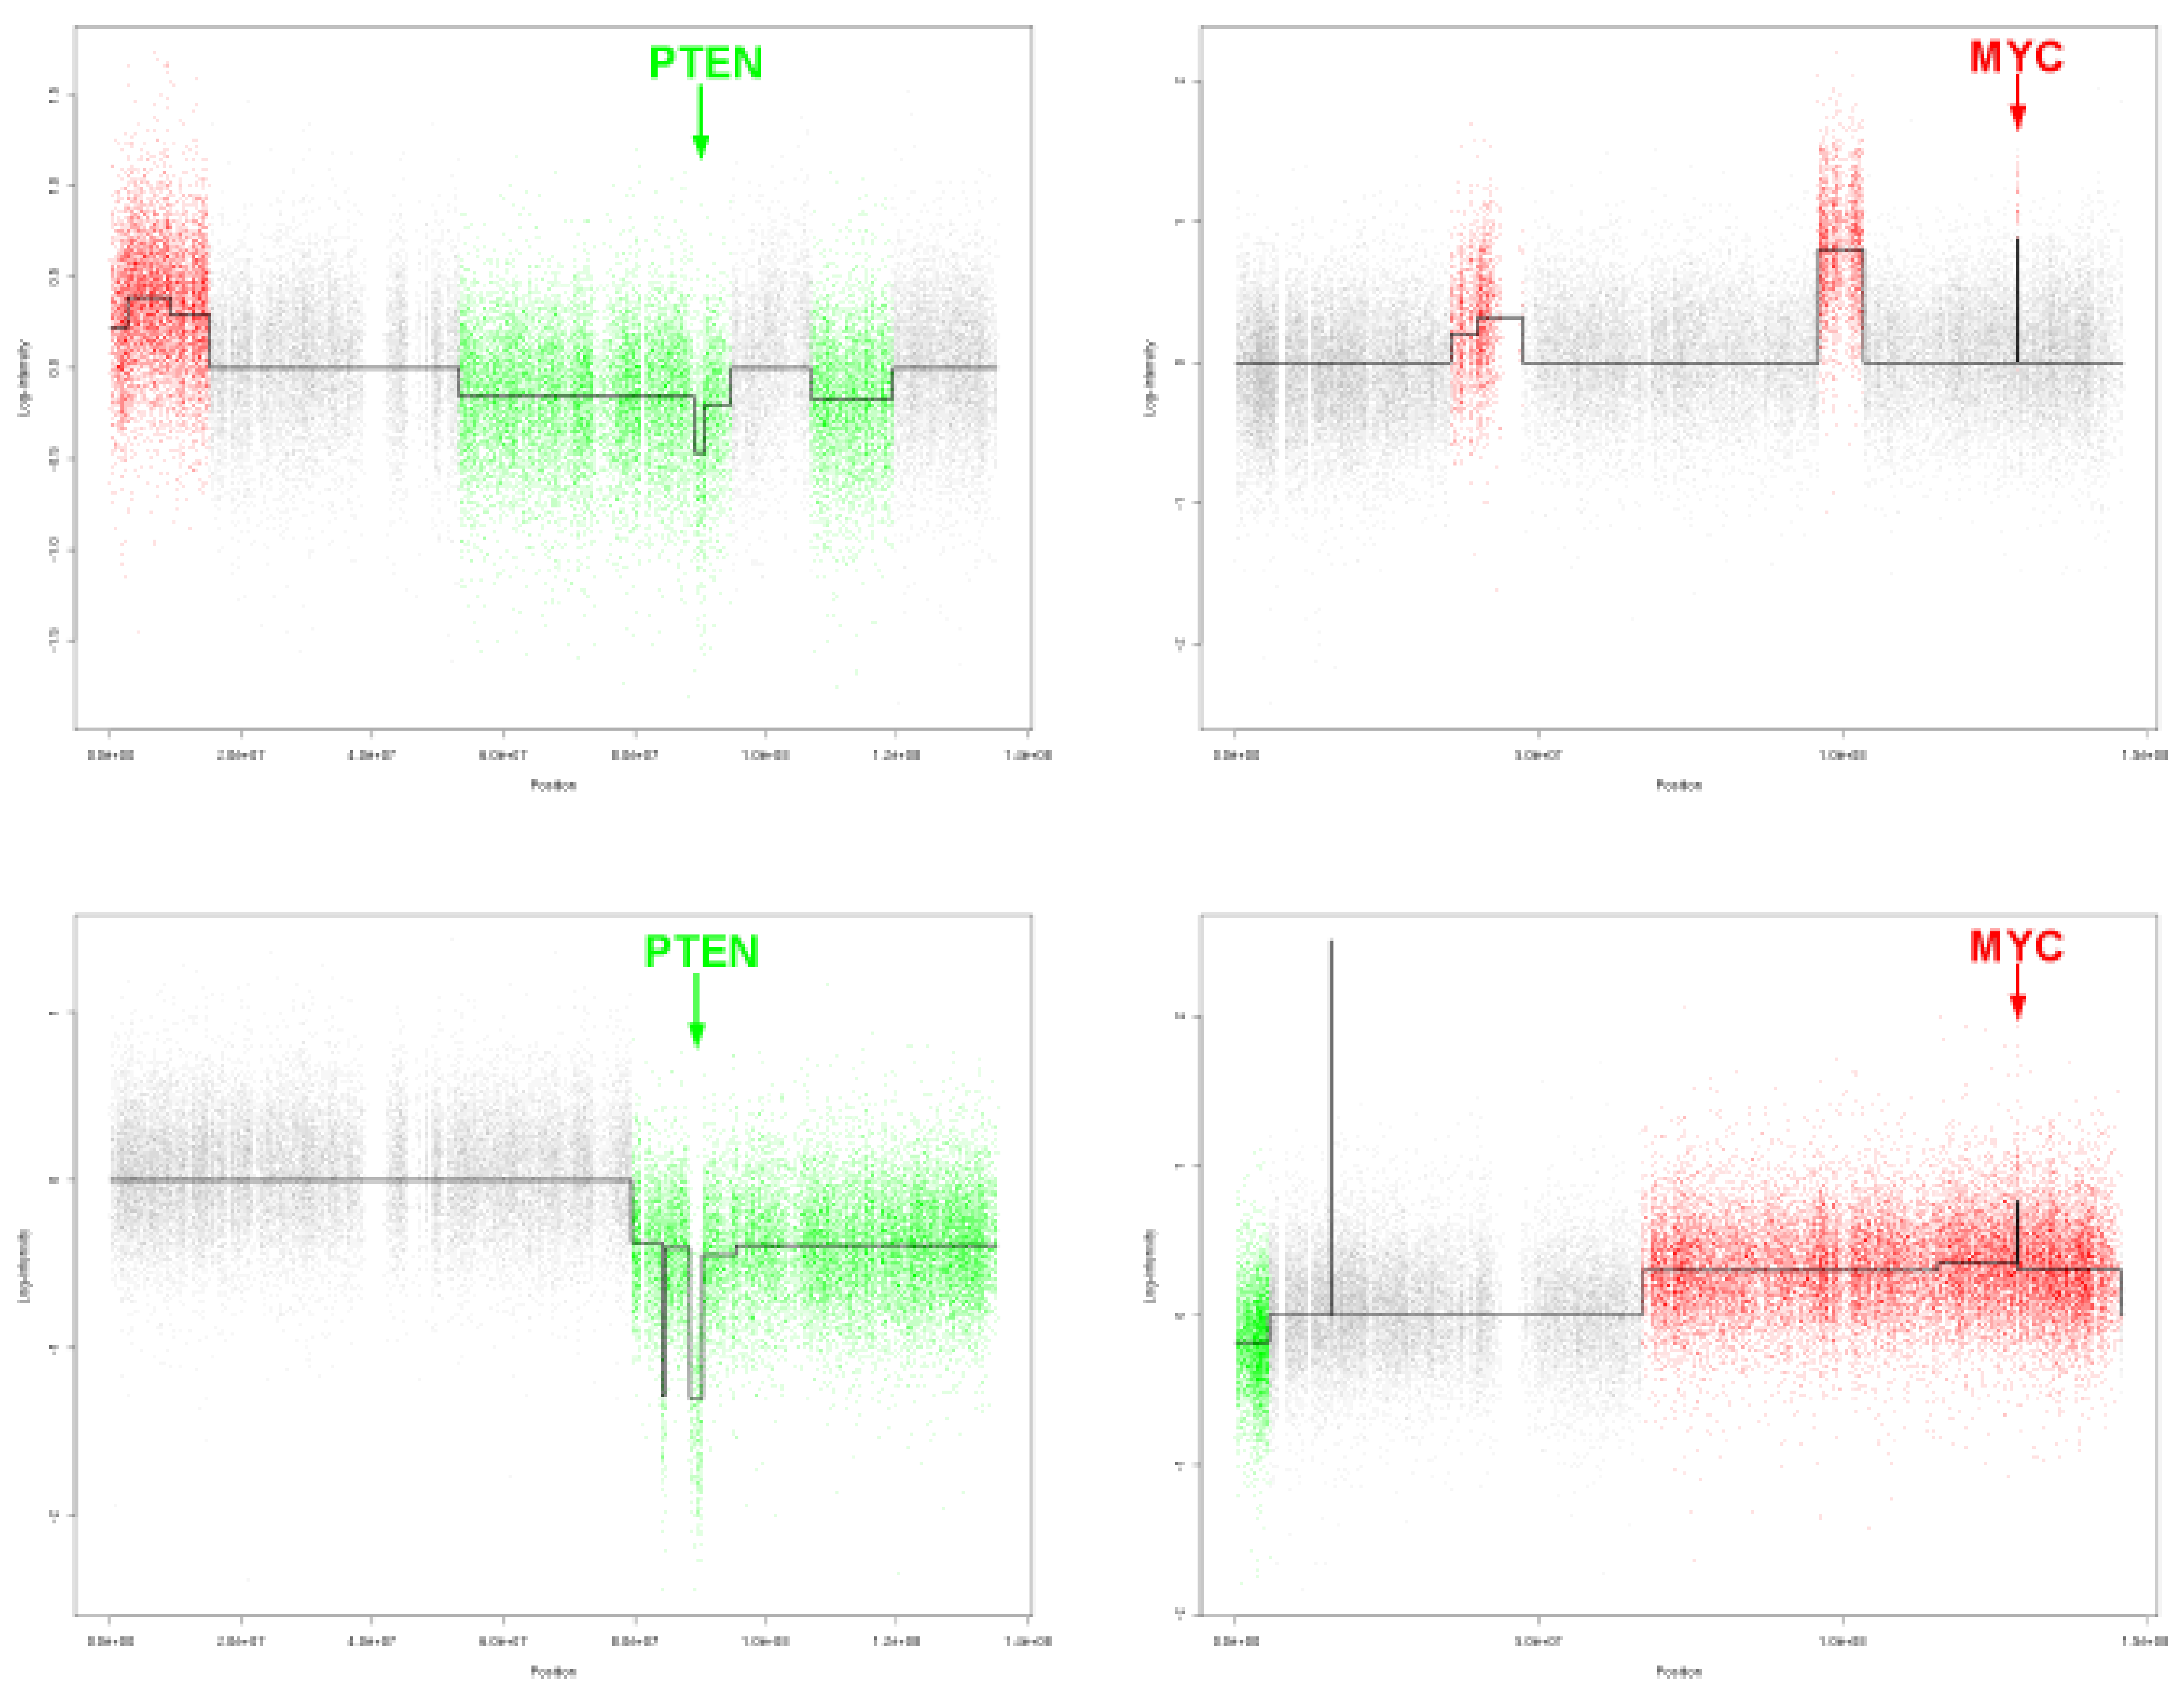
\includegraphics[height=.8\textheight]{../FIGURES/Rig10-Fig6-5}
  $$
  Chrom. 10 and 8 of two patients with breast carcinomas. \refer{Rig11} 
}

%====================================================================
\frame{\frametitle{Profiles}

  \begin{tabular}{cc}
    \begin{tabular}{p{0.5\textwidth}}
    \onslide+<1->{\paragraph{Individual profiles:} 
    patient $i$, locus $t$, 
    $$
    X_i(t) = \left\{
	 \begin{array}{ll}
	 0 & \text{if normal} \\
	 1 & \text{if \textcolor{red}{altered}}
	 \end{array}
    \right.
    $$
   }
    \onslide+<2->{\paragraph{Cumulated profile:}
    $$
    S_p(t) = \sum_{i=1}^p X_i(t)
    $$
    $= $ nb of altered patients at locus $t$ \\
   }
    \onslide+<3->{\bigskip
    \paragraph{Significance:}}
    \end{tabular}
    &
    \hspace{-0.1\textwidth}
    \begin{tabular}{c}
	 \begin{overprint}   
%	 \onslide<1>    
%	 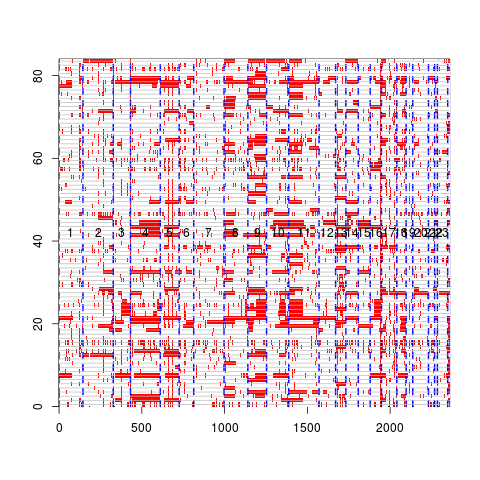
\includegraphics[height=.7\textheight, width=.5\textwidth]{../FIGURES/Fig-MinReg-Data-Prof} 
% 	 \onslide<2>    
% 	 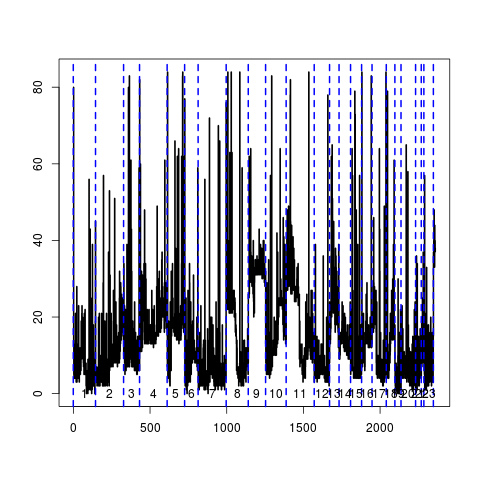
\includegraphics[height=.7\textheight, width=.5\textwidth]{../FIGURES/Fig-MinReg-Data-Cumul} 
	 \onslide<1>    
	 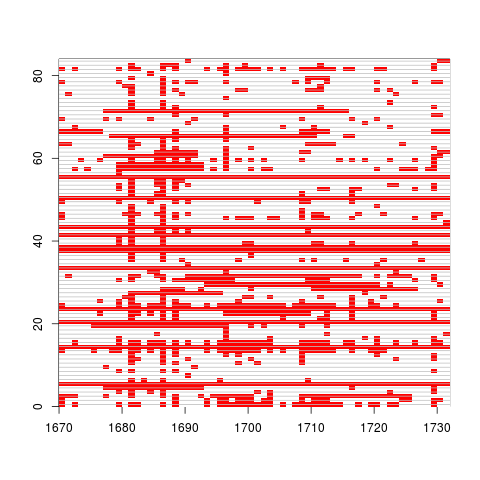
\includegraphics[height=.7\textheight, width=.5\textwidth]{../FIGURES/Fig-MinReg-Data-Prof13} 
	 \onslide<2>    
	 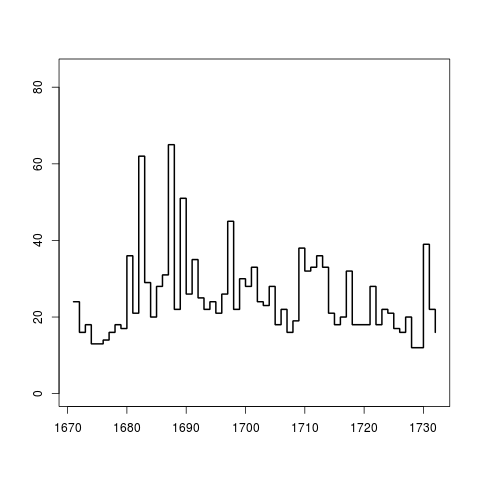
\includegraphics[height=.7\textheight, width=.5\textwidth]{../FIGURES/Fig-MinReg-Data-Cumul13} 
	 \onslide<3>    
	 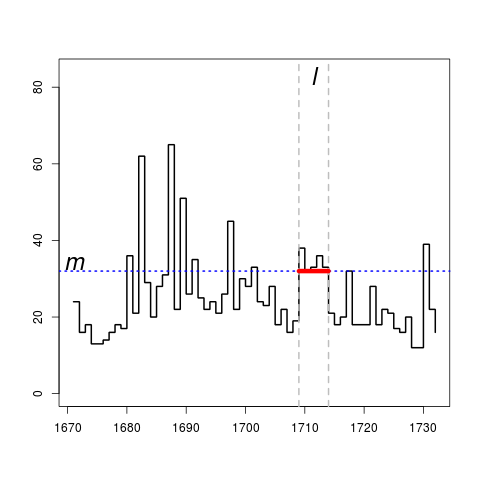
\includegraphics[height=.7\textheight, width=.5\textwidth]{../FIGURES/Fig-MinReg-Data-Reg1-13} 
	 \onslide<4>    
	 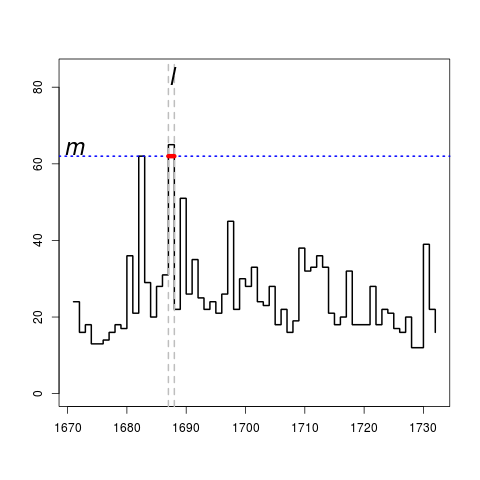
\includegraphics[height=.7\textheight, width=.5\textwidth]{../FIGURES/Fig-MinReg-Data-Reg2-13} 
	 \end{overprint}   
    \end{tabular}
  \end{tabular}
  \onslide+<3->{
  $$
  \pi(m, \ell) = \Pr\left\{\text{
  an excursion with length $\ell$ above level $m$ occurs
  }\right\}
  $$}

  }

%====================================================================
\frame{\frametitle{Generic null model}

  \paragraph{Individual profiles.} Define an \paragraph{homogeneous} (Markov) model for the profiles:
  $$
  X_i(t) \text{ iid } \sim F(\lambda, \mu) 
  $$
  $\lambda, \mu = $ e.g. alteration typical length and frequency.
  
  \bigskip \bigskip \pause
  \paragraph{Cumulated profiles.} Deduce the distribution of $S_p(t)$
  $$
  S_p(t) \sim G(\lambda, \mu)
  $$
  
  \bigskip \pause
  \paragraph{Significance.} Compute the probability of interest:
  $$
  \pi(m, \ell) =
  \Pr\left\{\text{$S_p(t)$ stays above the threshold $m$ for longer than $\ell$}\right\}
  $$
}

%====================================================================
\frame{\frametitle{Abacus}

  \paragraph{Significance isolines:} for given cohort size $p$, number of loci $n$ and parameter $\lambda, \mu \approx $ (mean nb. alterations, mean alteration length)
%   $$
%   \mathcal{C}_\alpha(\lambda, \mu) = \{(m, \ell): \pi(m, \ell) = \alpha\}
%   $$
%   (e.g. $\alpha = 1\%$) \vspace{-.1\textheight}
  $$
%   \vspace{-0.05\textheight}
  \begin{array}{rc}
    &   \text{For a given significance level $\alpha$ (e.g. 1\%):} \\
    \begin{array}{c} \rotatebox{90}{threshold $m$} \end{array} & 
    \begin{array}{c} 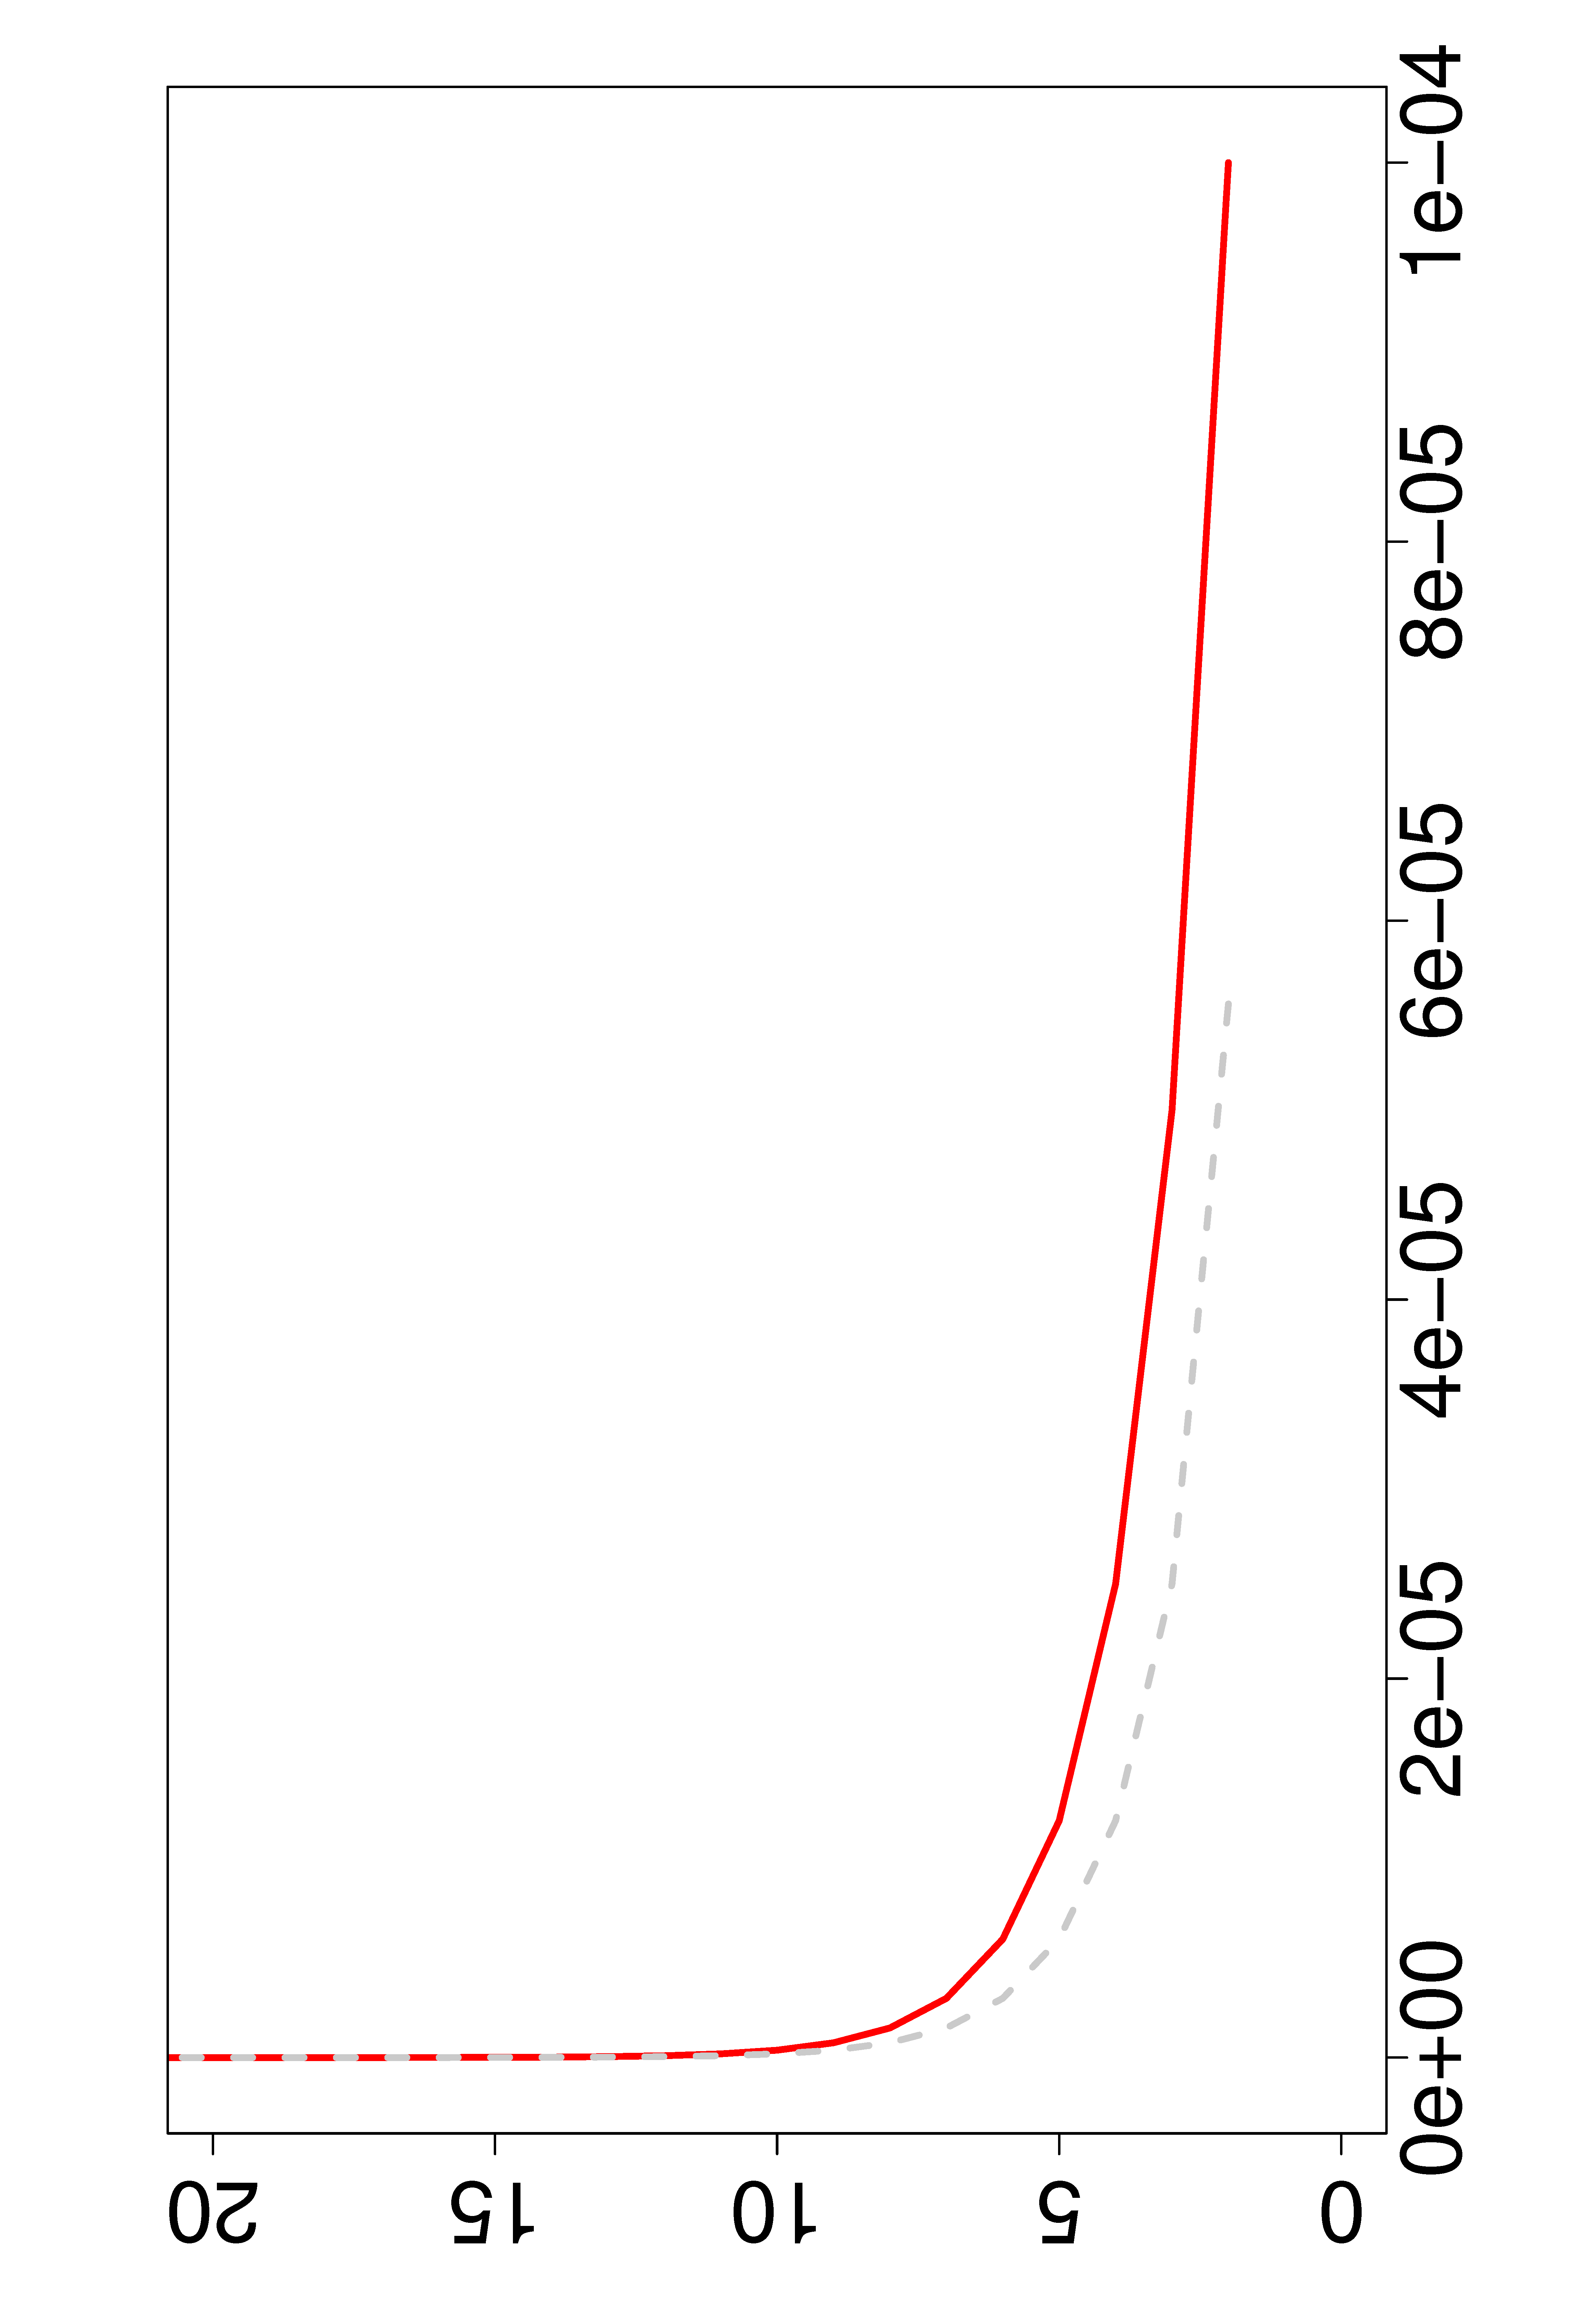
\includegraphics[height=.7\textheight, width=.45\textwidth, angle=270]{../FIGURES/Abaque-Example} \end{array} \\
    & \text{relative alteration length } \ell / n
  \end{array}
  $$
}

%====================================================================
\frame{\frametitle{Few loci, few patients}

  \paragraph{Mid 90' - early 00':} BAC arrays
  \begin{itemize}
   \item $10^3$ loci per array, $10^2$ loci per chromosome.
   \item $n \approx 10^2$ loci 
   \item $p \approx 10 - 10^2$ patients
  \end{itemize}
  
  \bigskip \bigskip \pause
  \paragraph{Probabilistic model:}
  \begin{itemize}
   \item Few loci $\rightarrow$ discrete 'time'
   \item Few patients $\rightarrow$ discrete 'state'
  \end{itemize}
}
  
%====================================================================
\frame{\frametitle{Discrete time Markov chain model}

  \paragraph{Individual profile = } stationary Markov chains over $\{0, 1\}$ with transition
  \begin{eqnarray*}
   0 & \rightarrow & 1: \quad \text{with probability } \lambda \\
   1 & \rightarrow & 0: \quad \text{with probability } \mu
  \end{eqnarray*}
%   $$
%   X_i(t) \sim MC(P_X), 
%   \qquad
%   P_X = \left( 
%     \begin{array}{cc} 1 - \lambda & \lambda \\ \mu & 1-\mu \end{array}
%   \right).
%   $$
  \ra Mean alteration length $= 1/ \mu$, one alteration every $\lambda\mu/(\lambda+\mu)$ locus.
  
  \bigskip \bigskip \pause
  \paragraph{Cumulated profile = } Markov chain over $\{0, \dots, p\}$ with transition
  $$
  S_p(t+1) | S_p(t) 
%   \quad \overset{\Delta}{=} \quad \underset{\text{stay altered}}{\mathcal{B}\left(S_p(t), 1-\mu \right)} \; + \; \underset{\text{become altered}}{\mathcal{B}\left(p-S_p(t), \lambda \right)}
  = \text{nb staying altered } + \text{nb becoming altered}
  $$
  \ra Transition matrix $P_S: (p+1) \times (p+1)$
}

%====================================================================
\frame{\frametitle{Embedded Markov chain\footnote{see \refer{Pru12} for a tutorial}}

%   \paragraph{Aim = compute $\pi(m, \ell)$.}
%   Define the stopping time 
%   $$
%   T(m, \ell) = \inf\{t: \forall u \in ]t-\ell, t], S_p(u) \geq m\},
%   $$
%   we have
%   $$
%   \pi(m, \ell) = \Pr\{T(m, \ell) \leq n\}.
%   $$
%   
%   \bigskip \pause
%   \paragraph{Embedded MC principle.} 
%   \begin{itemize}
%   \item Related to finite automata.
%   \item Construct a dedicated Markov chain with enlarged transition matrix $\Pt_S$ and an absorbing state that is reached at $T(m, \ell)$ \refer{FuL03}. 
%   \item In this case: relabel the states above $m$ to keep track of how long $S_p(t)$ has sojourned above $m$.
%   \end{itemize}
% }
% 
% %====================================================================
% \frame{\frametitle{Constructing $\Pt_S$}

%   \vspace{-.08\textheight}
  \begin{tabular}{cc}
    \begin{tabular}{p{0.3\textwidth}}
	 \paragraph{Example.}
	 $$
	 p = 20, m = 15, \ell = 4
	 $$

	 \onslide+<6->{
	 \bigskip
	 \paragraph{Result.}
	 $$
	 \pi(m, \ell) = 
% 	 \left[\Pt_S^{n-1}\right]_{S_p(1), \textcolor{red}{\mathbf{\dagger}}}
	\Pr\left\{\St(n) = \textcolor{red}{\mathbf{\dagger}}\right\}
	 $$
	 can be computed using the $\Pt_S$ matrix. \\ 
	 ~\\
	 \refer{RoS09}
	 }
    \end{tabular}
    &
%    \hspace{-0.05\textwidth}
    \begin{tabular}{c}
	 \begin{overprint}   
	 \onslide<1>  
	 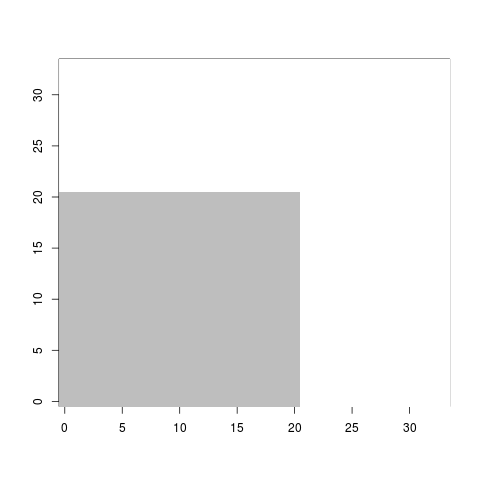
\includegraphics[height=.7\textheight]{../FIGURES/Fig-MinReg-EmbMC-Porg} \\
	 {\footnotesize $\{0, \dots, p\}$}
	 \onslide<2>    
	 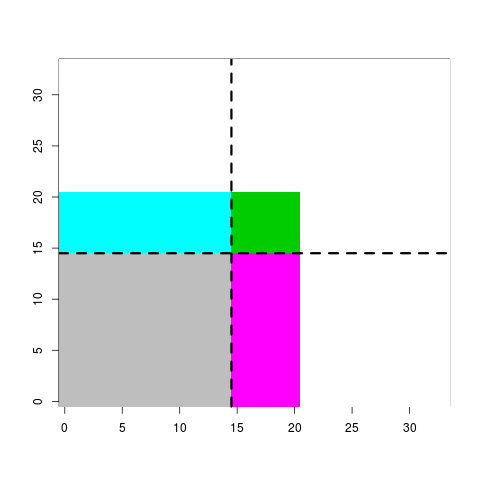
\includegraphics[height=.7\textheight]{../FIGURES/Fig-MinReg-EmbMC-Thres} \\
	 {\footnotesize $\{0, \dots, m-1, \underbrace{m, \dots, p}\}$}
	 \onslide<3>    
	 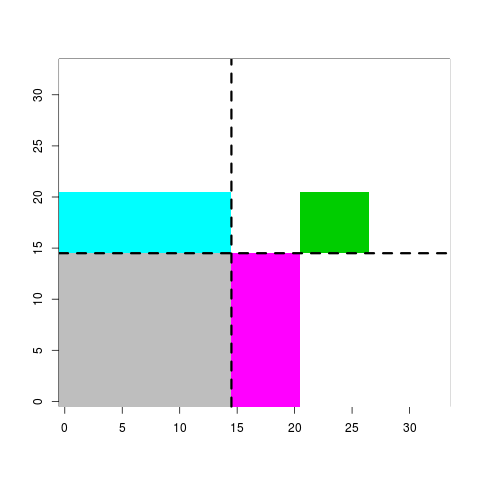
\includegraphics[height=.7\textheight]{../FIGURES/Fig-MinReg-EmbMC-1st} \\
	 {\footnotesize $\{0, \dots, m-1, \underbrace{m^1, \dots, p^1}, \underbrace{m^2, \dots, p^2}\}$}
	 \onslide<4>    
	 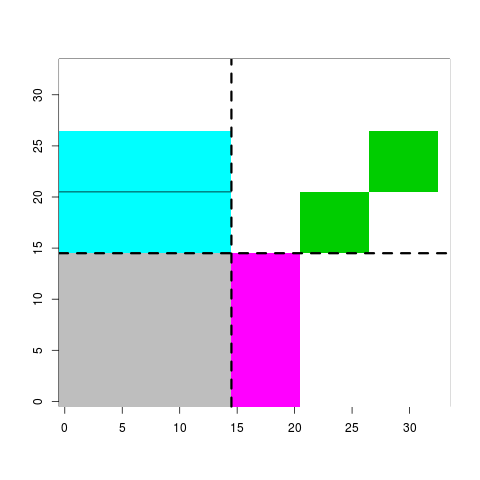
\includegraphics[height=.7\textheight]{../FIGURES/Fig-MinReg-EmbMC-2nd} \\
	 {\footnotesize $\{0, \dots, m-1, \underbrace{m^1, \dots, p^1}, \underbrace{m^2, \dots, p^2}, \underbrace{m^3, \dots, p^3}\}$}
	 \onslide<5>    
	 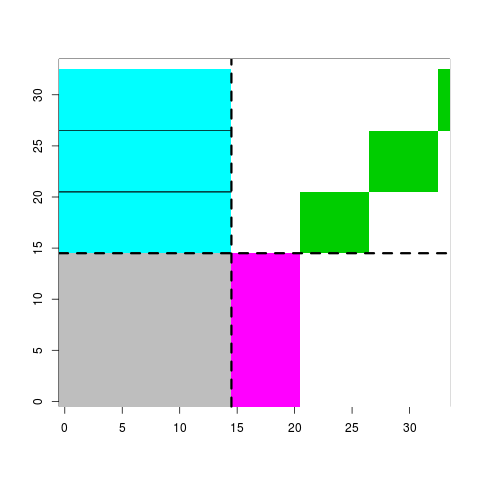
\includegraphics[height=.7\textheight]{../FIGURES/Fig-MinReg-EmbMC-3rd} \\
	 {\footnotesize $\{0, \dots, m-1, \underbrace{m^1, \dots, p^1}, \underbrace{m^2, \dots, p^2}, \underbrace{m^3, \dots, p^3}, \textcolor{red}{\mathbf{\dagger}}\}$}
	 \onslide<6->   
	 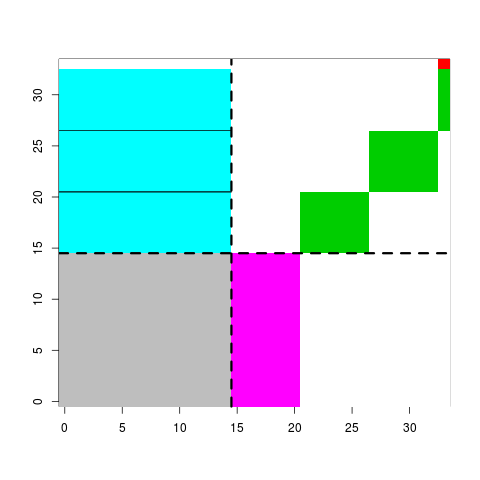
\includegraphics[height=.7\textheight]{../FIGURES/Fig-MinReg-EmbMC-Abs} \\
	 {\footnotesize $\{0, \dots, m-1, \underbrace{m, \dots, p}, \underbrace{m', \dots, p'}, \underbrace{m'', \dots, p''}, \textcolor{red}{\mathbf{\dagger}} \}$}
	 \end{overprint}   \\~
    \end{tabular}
  \end{tabular}

  
%   \onslide+<6>{
% %   \vspace{-0.1\textheight}
%   \ra Just need to compute $\Pt_S^{n-1}$.
%   }

  
%  \onslide+<7>{
%  \bigskip 
%  or, if $S_p(i) \sim \nu$,
%  $$
%  \pi(m, \ell) = \sum_s \nu(s) \pi_s(m, \ell) = \left[\nu^\top \Pt_S^{n-1}\right]_{\textcolor{red}{\mathbf{\dagger}}}
%  $$
%  }

  }

%====================================================================
\frame{\frametitle{(Provisional) conclusion}

  \paragraph{Ok:}
  \begin{itemize}
  \item Simple \& intuitive model,
  \item Exact result,
  \item Calculation easy to implement.
  \end{itemize}

  \pause \bigskip \bigskip
  \paragraph{But:}
  \begin{itemize}
  \item The embedded transition matrix $\Pt_S$ has dimension $\approx \ell \times p$ \\
  \ra not tractable for large cohorts and/or long alterations
  \item Computing its $n$-th power leads to numerical troubles for large number of loci. 
  \end{itemize}

  }

%====================================================================
\frame{\frametitle{SNP arrays: Many loci, few patients}

  \paragraph{Mid 00':} %CGH arrays, 
  SNP arrays
  \begin{itemize}
   \item $10^5-10^6$ loci per array, $10^4-10^5$ loci per chromosome.
   \item $n \approx 10^4-10^5 \rightarrow \infty$ loci
   \item $p \approx 10^2$ patients
  \end{itemize}
  
  \bigskip \bigskip \pause
  \paragraph{Probabilistic model:}
  \begin{itemize}
   \item Many loci $\rightarrow$ continuous 'time'
   \item Few patients $\rightarrow$ discrete 'state'
  \end{itemize}
}
  
%====================================================================
\frame{\frametitle{Births and deaths process}

  \paragraph{Individual profile = } stationary Markov processes over $\{0, 1\}$:
  \begin{eqnarray*}
   0 & \rightarrow & 1: \quad \text{rate } \lambda, \\
   1 & \rightarrow & 0: \quad \text{rate } \mu   
  \end{eqnarray*}
%   $$
%   \begin{array}{lll}
%    \text{rate} & 0 \rightarrow 1: & \lambda, \\
%    \text{rate} & 1 \rightarrow 0: & \mu,
%   \end{array}
%   \qquad \qquad
%   X_i(0) \sim \mathcal{B}\left(\frac{\lambda}{\lambda+\mu}\right).
%   $$
  \ra Same interpretation of $\lambda$ and $\mu$.
  
  \bigskip \bigskip \pause
  \paragraph{Cumulated profile = } births and deaths process over $\{0, \dots, p\}$ \\
%   with rates
%   \begin{eqnarray*}
%     s & \rightarrow & s+1: \quad \text{'birth' rate } \lambda \times (p-s) \\
%     s & \rightarrow & s-1: \quad \text{'death' rate } \mu \times s
%   \end{eqnarray*}
%   \ra infinitesimal generator (transition rates) $Q_S: (p+1) \times (p+1)$. \\
%   
%   \bigskip \pause
%   \paragraph{Pb:} The embedded Markov chain approach does not apply anymore.
  ~\\
  \ra Continuous time process (no 'next' locus)
}

%====================================================================
\frame{\frametitle{Stopping time}

  \bigskip
  $T(m, \ell) = $ First time $t$ when $S_p$ has just passed a time $\ell$ above the threshold $m$. 
  \bigskip \pause
  \begin{tabular}{cc}
    \begin{tabular}{p{0.3\textwidth}}
%  	 \onslide+<2->{$\ell = .05$} \\
 	 \onslide+<2->{Given $\ell$ and $m$} \\
 	 \onslide+<3->{$A = T_{S_p(0) \rightarrow m}$} \\
	 \onslide+<4->{$B = (T_{m \rightarrow m-1} | < \ell)$} \\
	 \onslide+<5->{$C = T_{m-1 \rightarrow m}$} \\
    \end{tabular}
    &
    \hspace{-0.1\textwidth}
    \begin{tabular}{p{0.5\textwidth}}
	 \begin{overprint}   
	 \onslide<2>    
	 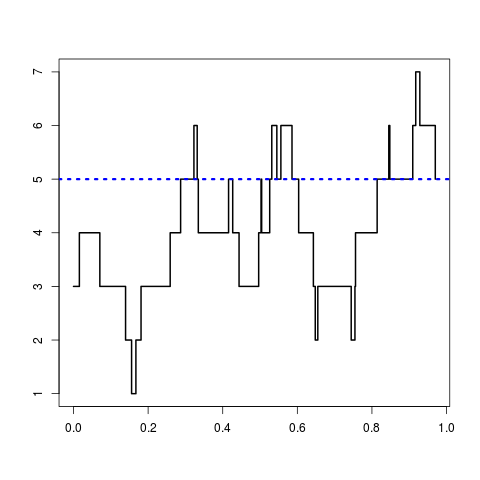
\includegraphics[height=.65\textheight, width=.65\textwidth]{../FIGURES/Fig-MinReg-BirDea-Thres} 
	 \onslide<3>    
	 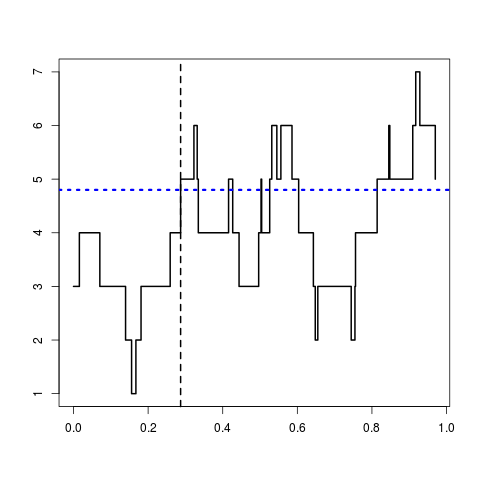
\includegraphics[height=.65\textheight, width=.65\textwidth]{../FIGURES/Fig-MinReg-BirDea-Time1}
	 \onslide<4>    
	 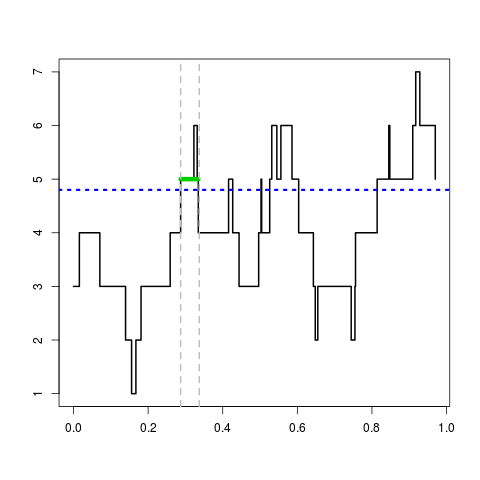
\includegraphics[height=.65\textheight, width=.65\textwidth]{../FIGURES/Fig-MinReg-BirDea-Excur1} 
	 \onslide<5>    
	 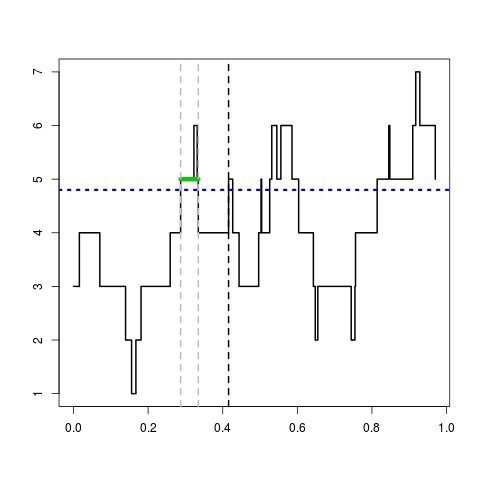
\includegraphics[height=.65\textheight, width=.65\textwidth]{../FIGURES/Fig-MinReg-BirDea-Time2} 
	 \onslide<6>    
	 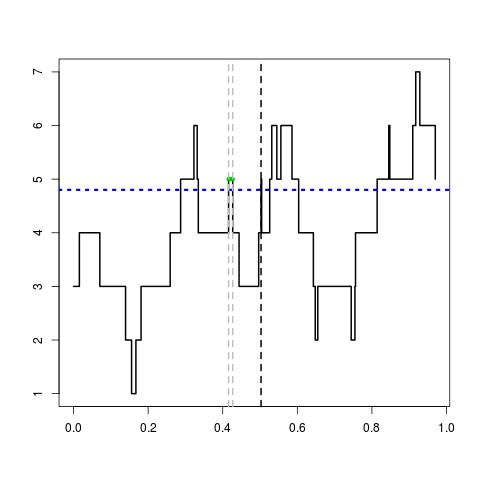
\includegraphics[height=.65\textheight, width=.65\textwidth]{../FIGURES/Fig-MinReg-BirDea-Time3} 
	 \onslide<7>    
	 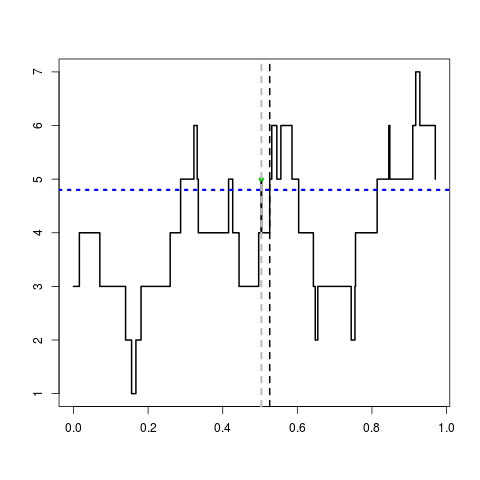
\includegraphics[height=.65\textheight, width=.65\textwidth]{../FIGURES/Fig-MinReg-BirDea-Time4} 
% 	 \onslide<8>    
% 	 \includegraphics[height=.65\textheight, width=.65\textwidth]{../FIGURES/Fig-MinReg-BirDea-Time5} 
	 \onslide<8->    
	 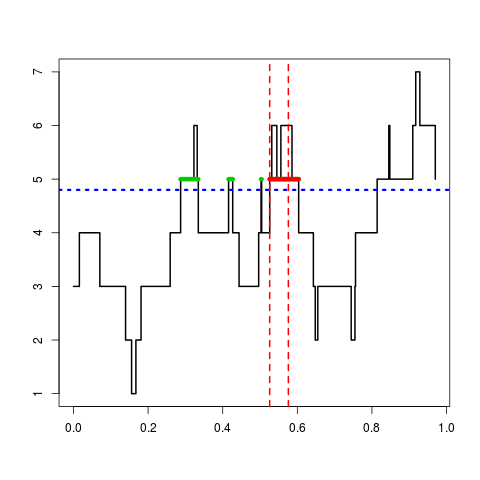
\includegraphics[height=.65\textheight, width=.65\textwidth]{../FIGURES/Fig-MinReg-BirDea-OK} 
	 \end{overprint} 
    \end{tabular}
  \end{tabular}
  \vspace{-.15\textheight}
  \begin{center}
  \onslide+<2->{$T(m, \ell) = $}
  \onslide+<3->{$A$} 
  \onslide+<4->{$+ B_1$} 
  \onslide+<5->{$+ C_1$} 
  \onslide+<6->{$+ (B_2 + C_2)$} 
  \onslide+<7->{$+ (B_3 + C_3)$} 
%   \onslide+<8->{$+ (B_4 + C_4)$} 
  \onslide+<8->{$+ \ell$}
  \end{center}

  \refer{RoS13}
  }

% %====================================================================
% \frame{\frametitle{Laplace transform of the stopping time}
% 
% %   \paragraph{Birth and death process.} 
% %   \begin{itemize}
% %    \item Hitting time: $T_{a \rightarrow b} =$ First time $S_p$ reaches $b$ starting from $a$.
% %    \item \refer{BaS01} provide the Laplace transform of all hitting times $\phi_{T_{a \rightarrow b}}(u)$.
% %    \item Laplace transforms are convenient to handle sums of r.v.'s like
% %    $$
% % %    T(m, \ell) = A + (B_1 + C_1) + (B_2 + C_2) + (B_3 + C_3) + (B_4 + C_4) + \ell
% %    T(m, \ell) = A + (B_1 + C_1) + (B_2 + C_2) + (B_3 + C_3) + \ell
% %    $$
% %   \item Number of trials $\sim$ geometric dist. with parameter $\Pr\{T_{m \rightarrow m-1} \geq \ell\}$
% %   \end{itemize}
%   
%   \paragraph{Probabilistic tool.} The waiting time is defined as a sum of random variables:
%    $$
%    T(m, \ell) = A + (B_1 + C_1) + (B_2 + C_2) + (B_3 + C_3) + \ell
%    $$
%    the Laplace transform of which can be derived.
% 
%   \bigskip \bigskip \pause
%   \paragraph{Result.} 
%   \begin{itemize}
%    \item A nice formula for the Laplace transform $\Phi_{T(m, \ell)}$
%    \item That you need to invert to get
%   $$
%   \Pr\{T(m, \ell) \leq n\} = \Phi^{-1}_{T(m, \ell)}(n),
%   $$
%   which can be done numerically using e.g. \refer{AbW06}.
%   \end{itemize}
%   }

%====================================================================
\frame{\frametitle{(Provisional) conclusion}

  \paragraph{Ok:}
  \begin{itemize}
  \item Simple \& intuitive model,
  \item Exact result (up the continuous approximation).
  \end{itemize}

  \pause \bigskip \bigskip
  \paragraph{But:}
  \begin{itemize}
  \item The inversion of the Laplace transform is numerically unstable \\
  \ra not usable in practice large cohort size $p$
  \end{itemize}

  }

%====================================================================
\frame{\frametitle{DNAseq: Many loci, many patients}

  \paragraph{Mid 00':} NGS, DNA-seq
  \begin{itemize}
   \item $10^9$ nucleotides per genome, $10^7-10^8$ nucleotides per chromosome.
   \item $n \rightarrow \infty$ loci
   \item $p \approx 10^3-10^4 \rightarrow \infty$ patients
  \end{itemize}
  
  \bigskip \bigskip \pause
  \paragraph{Probabilistic model:}
  \begin{itemize}
   \item Many loci $\rightarrow$ continuous 'time'
   \item Many patients $\rightarrow$ continuous 'state'
  \end{itemize}

  \bigskip
  \Refer{On-going work} %: Decreusefond, Etienne, Lang, R., Vallois}
}
  
%====================================================================
\frame{\frametitle{Ornstein-Uhlenbeck process}

  \paragraph{Individual profile =} same continuous time Markov processes as before.
  
  \bigskip \pause
  \paragraph{Cumulated profile \ra} diffusion process as $p$ goes ton infinity:

  \bigskip 
  \begin{proposition} 
%   Denoting $\tau = \lambda + \mu$, $\theta = \lambda/\tau$, $\sigma^2 = \theta(1-\theta)$,
%   $$
%   \St_p(t) := \frac{S_p(t) - p \theta}{\sigma \sqrt{p}} 
%   \quad \overset{\Delta}{\underset{p \rightarrow \infty}{\longrightarrow}} \quad 
%   Z(t)
%   $$
%   where $Z(t) \sim OU(\tau)$ is a stationary Ornstein-Uhlenbeck process with zero mean, unit
%   variance and recall parameter $\tau$:
%   $$
%   \dd Z(t) = - \tau Z(t)  \dd t + \dd B(t).
%   $$
  The normalized version of $S_p(t)$ converges to an Ornstein-Uhlenbeck (OU) process.
  \end{proposition}
}

% %====================================================================
% \frame{\frametitle{Convergence of the longest excursion}
% 
%   \paragraph{The longest excursion} is not a continuous function of the path, so sufficient to guaranty the convergence in distribution so 
%   $$
%  \St_p(t) \overset{\Delta}{\longrightarrow}
%   OU(\tau)
%   $$
%   is not sufficient to prove that 
%   $$
%   V^{(1)}_{\St_p} \overset{\Delta}{\longrightarrow} V^{(1)}_{OU(\tau)}.
%   $$
%   
%   \bigskip \pause
%   Still, denoting $\St_p^{-\ell}(t) = \min_{t-\ell \leq u \leq t} \St_p(u)$, we have that
%   $$
%   \pi(m, \ell) = 
%   \Pr\left\{\max_{\ell \leq t \leq n} \St_p^{-\ell}
%   (t) \geq \mt\right\}
%   $$  
%   so the convergence of $V^{(1)}_{\St_p}$ holds.
% }

%====================================================================
\frame{\frametitle{New version of the problem}

  \bigskip
  Denote $V_{OU}(\mt)$ the longest excursion of an $OU(\tau)$ above threshold $\mt$:
  $$
  \pi(m, \ell) = \Pr\{V_{OU}(\mt) \geq \ell\}.
%   , \qquad \mt = (m-p\theta)/\sigma\sqrt{p}.
  $$
  
  $$
  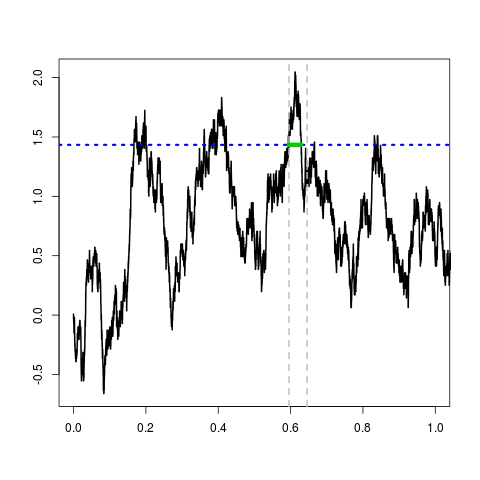
\includegraphics[height=.65\textheight, width=.7\textwidth]{../FIGURES/Fig-MinReg-Diffus-Longest} 
  $$
  }

%====================================================================
\frame{\frametitle{Distribution of the longest excursion of an $OU$ process}
  
  \paragraph{Problem:} Few is known about the longest excursion of an $OU$ process...

  \bigskip \pause
  \paragraph{But} 
%   \begin{itemize}
%    \item \refer{PiY97} provide a (simple) way to sample the lengths of the excursions of a Brownian motion $V^{(1)}_B \geq V^{(2)}_B \geq \dots$ (+ some other relevant quantities).
%    \item 
   \refer{PiY97} provide a (simple) way to sample the excursions $V_B$ of a Brownian motion
%    \item \refer{APP05} provides the distribution of the hitting time $T_{\mt}$ for an OU process.
%   \end{itemize}

  \bigskip \pause
  \paragraph{Importance sampling.}
  \begin{itemize}
   \item Sample a large number of sets of Brownian excursion lengths $\{V_B\}$.
   \item Re-weight each of them according to ${\dd P_{OU}}/{\dd P_B}$ (Girsanov formula).
  \end{itemize}
}

% %====================================================================
% \frame{\frametitle{Importance sampling}
% 
% \onslide+<1->
% {We know how to sample $V^{(n)}_B$ but not \textcolor{red}{$V^{(n)}_{OU}$}. \\}
% 
%   \begin{tabular}{cc}
%     \begin{tabular}{p{.4\textwidth}}
% 	 \begin{enumerate}
% 	 \onslide+<2->
% 	 {\item Sample a large number $N$ of copies $V^{(n)}_{B, 1}$, $V^{(n)}_{B, 2}$, \dots, $V^{(n)}_{B, N}$. \\ ~}
% 	 \onslide+<3->
% 	 {\item Reweight each $V_{B, j}$ with 
% 	 $$
% 	 w_j \propto \textcolor{blue}{{\dd P_{OU}}/{\dd P_B}(V_{B, j})}.
% 	 $$}
% 	 \end{enumerate}
% 	 \onslide+<4->
% 	 {$$
% 	 \widehat{\pi}(m, \ell) = \frac{\sum_j w_j \mathbb{I}\{W_{B, j} > \ell\}}{\sum_j w_j}
% 	 $$}
%     \end{tabular}
%     &
%     \hspace{-.05\textwidth}
%     \begin{tabular}{c}
%      \begin{overprint}
%       \onslide<1>
%      	 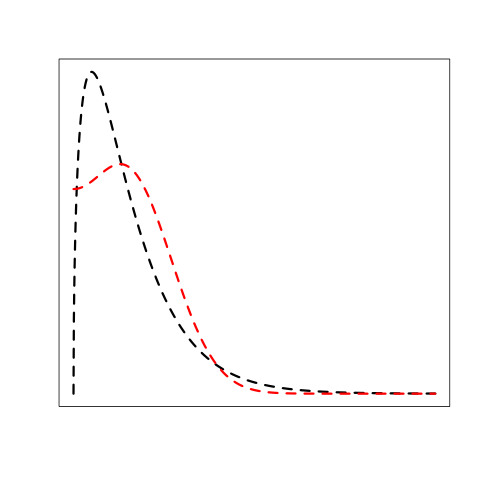
\includegraphics[scale=.4]{../FIGURES/Fig-MinReg-Diffus-ImpSamp0} 
%       \onslide<2>
%      	 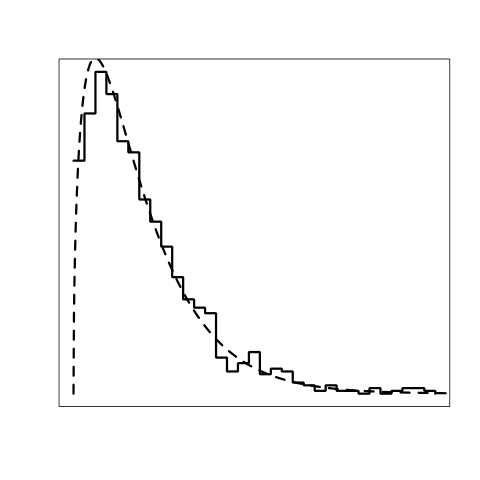
\includegraphics[scale=.4]{../FIGURES/Fig-MinReg-Diffus-ImpSamp2} 
%       \onslide<3>
%      	 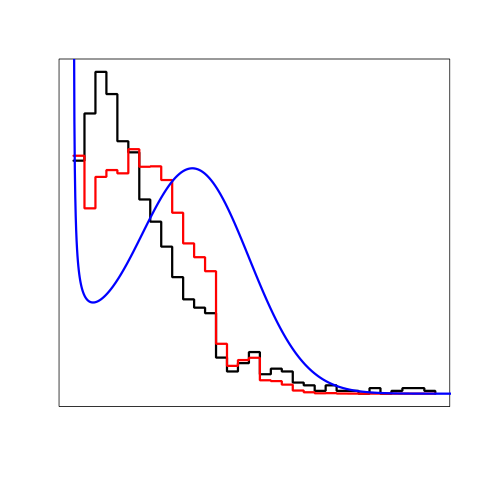
\includegraphics[scale=.4]{../FIGURES/Fig-MinReg-Diffus-ImpSamp3} 
%       \onslide<4->
%      	 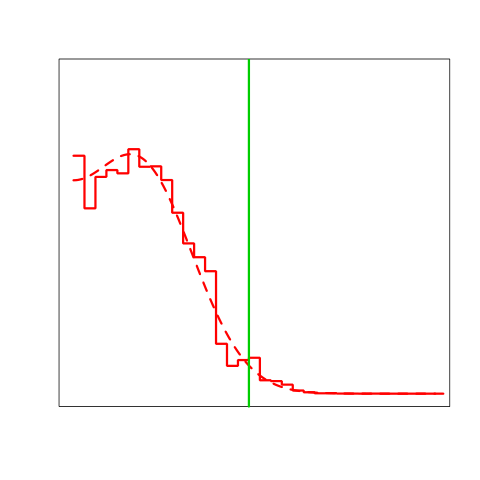
\includegraphics[scale=.4]{../FIGURES/Fig-MinReg-Diffus-ImpSamp4} 
%      \end{overprint}
%     \end{tabular}
%   \end{tabular}
%   
% %   \vspace{-.05\textheight}
% %   \onslide+<5>{A sampling scheme can be designed to sample $OU$ excursions.}
% 
% }
% 
% %====================================================================
% \frame{\frametitle{A theoretical issue}
% 
%   \vspace{-.05\textheight}
%   \begin{tabular}{cc}
%     \begin{tabular}{p{.4\textwidth}}
% 	 \paragraph{The longest excursion} is not a continuous function so 
% 	 $$
% 	 \St_p \overset{\Delta}{\longrightarrow} OU(\tau)
% 	 $$
% 	 is not enough to prove that 
% 	 $$
% 	 V^{(1)}_{\St_p} \overset{\Delta}{\approx} V^{(1)}_{OU(\tau)}.
% 	 $$
%     \end{tabular}
%     &
%     \hspace{-.1\textwidth}
%     \begin{tabular}{c}
%      	 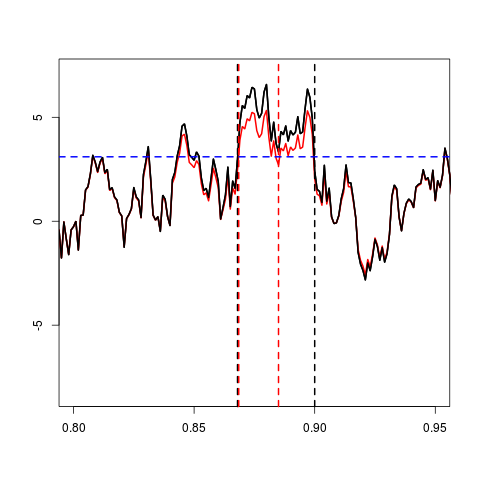
\includegraphics[width=.6\textwidth, height=.55\textheight]{../FIGURES/Fig-MinReg-Diffus-Continuity}      
%     \end{tabular}
%   \end{tabular} \\
%   \pause
%   Still, the problem can be reformulated as
%   $$
%   \pi(m, \ell) = \Pr\left\{\max_{\ell \leq t \leq n} \St_p^{-\ell}(t) \geq \mt\right\}
%   $$
%   where $\St_p^{-\ell}(t) = \min_{t-\ell \leq u \leq t} \St_p(u)$, which relies on continuous transforms\footnote{Many thanks to P. Vallois.}.
%   
% %   $\St_p \overset{\Delta}{\longrightarrow} OU(\tau)$
% %   means that, for any continuous function $f$:
% %   $$
% %   \mathbb{E}[f(\St_p)] \underset{p \rightarrow \infty}{\longrightarrow}  \mathbb{E}[f(OU(\tau))].
% %   $$
% %   \vspace{-.05\textwidth}
% %   \begin{tabular}{cc}
% %     \begin{tabular}{p{.4\textwidth}}
% % 	 \paragraph{The longest excursion} of $\St_p$ above $\mt$ is a (measurable) function \dots \\
% % 	 ~\\
% % 	 but it is not continuous.
% %     \end{tabular}
% %     &
% %     \hspace{-.05\textwidth}
% %     \begin{tabular}{c}
% %      	 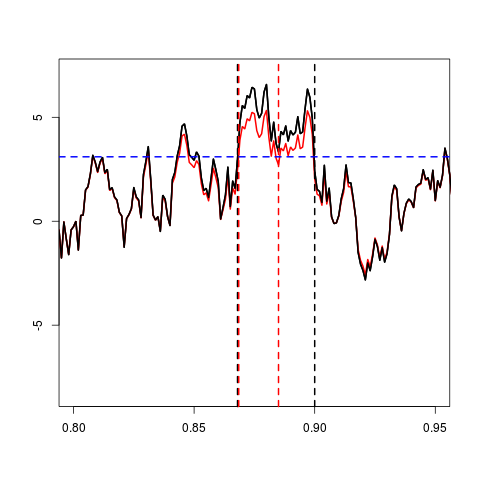
\includegraphics[scale=.4]{../FIGURES/Fig-MinReg-Diffus-Continuity}      
% %     \end{tabular}
% %   \end{tabular}
% 
% }
% 
%====================================================================
\frame{\frametitle{(Provisional) conclusion}

  \paragraph{Pros:}
  \begin{itemize}
  \item An exact importance sampling scheme can be designed \\
  \item The approximation can handle arbitrary loci density $n$ and number of patients $p$ \\
  \ra 'scalable' approach for next sequencing technologies ($n \approx 10^8$)
  \item Abacus can be computed \paragraph{once for all}.
  \end{itemize}

  \pause \bigskip \bigskip
  \paragraph{But:}
  \begin{itemize}
%   \item The proposed sampling strategy still needs to be implemented in practice...
  \item The efficiency of the preferential sampling scheme is critical.
%   \item   We have no theoretical guarantee that the longest excursion of the process of interest behaves like this of an Ornstein-Uhlenbeck process.
%   \item In the worst case, the proposed approach is useless.
  \end{itemize}

  }

%====================================================================
\section*{Concluding remarks}
\frame{\frametitle{Concluding remarks}}

%====================================================================
\frame{\frametitle{Segmentation problems in genomics}

 
  \hspace{-.05\textwidth}
  \begin{tabular}{cc}
    \begin{tabular}{p{.5\textwidth}}
    \paragraph{All over the place:}
    \begin{itemize}
     \item Looking for genomic regions with correlated expression \refer{DLM15}
     \item Understanding genomic 3D interactions with HiC \refer{LDM14}
    \end{itemize}
    
    \bigskip
    \paragraph{Same recurrent issues:}
    \begin{itemize}
     \item Data modeling
     \item Algorithmic efficiency
     \item Model selection
    \end{itemize}

    \end{tabular}
    & 
    \hspace{-.075\textwidth}
    \begin{tabular}{c}
    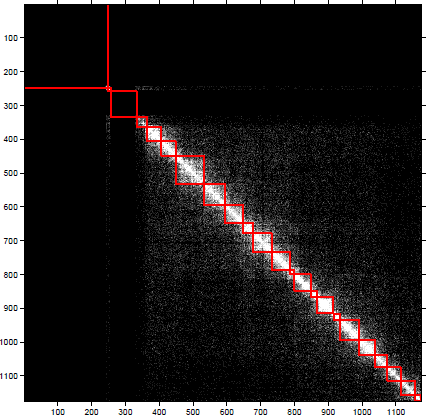
\includegraphics[width=.45\textwidth]{\fighd/LDM14-ECCB-Fig2b}
    \end{tabular}
  \end{tabular}
  
  \bigskip
  \paragraph{NGS = critical advances?} ~\\
  Data collected at the nucleotide level $=$ 'atomic' resolution for genomics.
}


%====================================================================
\frame{\frametitle{Co-authors}

%   \paragraph{Joint (on-going) work with}
  
  \begin{enumerate}
   \item A. Cleynen, E. Lebarbier, F. Picard, G. Rigaill, \\~
   \item L. Decreusefond\footnote{from TelecomParisTech}, M.-P. Etienne, G. Lang, V. Stefanov, P. Vallois
  \end{enumerate}
}

%====================================================================
%====================================================================
\subsection*{References}
%====================================================================
{\tiny
  \bibliography{/home/robin/Biblio/ARC,/home/robin/Biblio/AST,/home/robin/Biblio/SSB}
%   \bibliographystyle{/home/robin/LATEX/Biblio/astats}
  \bibliographystyle{plain}
  }
  
%====================================================================
\frame{\frametitle{Some R packages}

  \paragraph{CGHseg:} Comprehensive package for joint segmentation of multiple profile (+ between profiles correlation + bias correction + calling) 
  
  \bigskip
  \paragraph{EBS:} Exact posterior distribution for segmentation (model selection, credibility intervals, ...) for both microarray and NGS 

  \bigskip
  \paragraph{Segmentator3IsBack:} Pruned dynamic programming for efficient segmentation of large signals (microarray, NGS) 

  \bigskip
  \paragraph{HiCseg:} Segmentation method for the analysis of HiC data (cis-interaction)
  
  \bigskip\paragraph{SegCorr:} Correlation matrix segmentation for the detection of highly correlated expression regions
}

%====================================================================
%====================================================================
\end{document}
%====================================================================
%====================================================================

